\chapter{Railway Network Analyzer (RNA)}
    \label{sec:RNA}

    El sistema ferroviario consta de diversos elementos que incluyen la infraestructura, sensores, actuadores  e interfaces visuales con los conductores. Todos estos elementos se interrelacionan y funcionan en conjunto dentro del sistema de señalamiento y el sistema de enclavamiento. Cada uno de estos elementos y como se relacionan se encuentran definido en el formato railML. 

    El RNA deberá procesar cualquier archivo compatible con railML [REF], detectar cada elemento junto a sus propiedades y como están conectados dentro de la red ferroviaria. En base a esta información, que define la infraestructura, es decir, las características estáticas de la red, el RNA deberá detectar los puntos críticos. Es decir, las zonas en las cuales es mas probable que ocurran colisiones entre formaciones, ya sea de frente como lateralmente, así como también los descarrillamientos. Cada elemento ferroviario, según corresponda a cada elemento, será protegido por una serie de semáforos. La conjunción de todos estos semáforos probablemente dará lugar a superposiciones o contradicciones que luego serán simplificadas por el RNA antes de su resultado final.

    En base al señalamiento generado, el RNA debe detectar todas las rutas posibles y generar una nueva tabla de enclavamientos. De existir un señalamiento previo, deberá compararlos y verificar que todas las rutas originales pueden ser generadas combinando una o mas de las rutas nuevas. Adicionalmente, el RNA validará que el señalamiento cumple los principios establecidos en la Sección \ref{sec:principios} y que la sintaxis del archivo railML obtenido es correcta.    

    \section{Biblioteca RailML}

    El primer paso en el desarrollo del RNA es contar con una librería que permita generar un objeto equivalente uno a uno con el estándar railML y luego exportar un nuevo archivo railML. Como ya se mencionó en la Sección \ref{sec:railML}, el estándar railML define cinco clases de objetos principales: Common, Infraestructure, Interlocking, RollingStock y Timetable. 

    La clase Common incluye 109 subclases, todas ellas utilizadas para definir características generales e invariantes para la red. Por ejemplo, podemos encontrar la clase Concessionaire que define quien tiene la concesión de la red, la clase tBrakeType que define el tipo de frenos aceptados en esa red, la clase tVoltage que define la tensión de la red o la clase PublicHolidayPeriodRule que define el período de vacaciones de los operarios de la red, entre otros factores. Esta clase es obligatoria para todos los archivos en formato railML, por lo tanto es necesaria para el funcionamiento del RNA, aunque no se extraigan datos importantes de la misma.

    La clase Infraestructure incluye  231 subclases, todas ellas enfocadas en definir las características estáticas de cada elemento ferroviario, como su posición, dimensiones y demás parámetros invariantes en el tiempo.  Entre ellas podemos encontrar la clase Borders (ver Sección XX), BufferStops (ver Sección XX), LevelCrossingsIS (ver Sección XX), Platforms (ver Sección XX), SignalsIS (ver Sección XX), SwitchesIS (ver Sección XX) y Tracks (ver Sección XX), entre otras. Adicionalmente incluye dos clases fundamentales para el análisis de redes de grafos: netElement y netRelation, ambas discutidas en la Sección XX. En el caso de hacer análisis a nivel meso y macroscópico se tienen, además, las clases Line, OperationalPoint y Network, no cubiertas en este análisis.

    La clase Interlocking incluye 156 subclases, todas ellas enfocadas en definir las características dinámicas de los elementos ferroviarios que las posean. Entre ellas podemos encontrar LevelCrossingsIL (ver Sección XX), SignalsIL (ver Sección XX), SwitchesIL (ver Sección XX), entre otras. Adicionalmente, se encuentras las subclases relacionadas a la tabla de enclavamientos y las rutas, como Routes, CombinedRoutes, ConflictingRoutes, RoutesRelations y muchas otras referidas explícitamente a rutas (ver Sección XX). 
    
    El RNA solamente necesita de las clases Common, Infraestructure e Interlocking para funcionar, por lo que no fue necesario implementar las clases RollingStock ni Timetable. En total se han implementado 524 clases, considerando 28 clases nativas de RailTopoModel necesarias para que railML pueda interpretar los tipos de datos definidos. Todas las clases y subclases mencionadas son opcionales en el estándar, salvo que se indique lo contrario, es decir, no son obligatorias para que el archivo railML se considere válido.

    En las siguientes secciones se detallaran las subclases mas importantes implementadas, tal que se pueda comprender que atributos son procesados para poder generar el señalamiento. Se comenzará con las clases relativas a la topología de la red, eje central análisis del RNA y se proseguirá con las clases asociadas a elementos ferroviarios materiales. Simultáneamente, se profundizará en los conceptos mas destacados de cada elemento ferroviario correspondiente a esa clase, destacando cual es el señalamiento asociado al mismo para protegerlo en base a los principios ferroviarios expuestos.

    % COMMON
    \subsection{Campo de metadatos}
    \label{sec:metadata}

    Aunque no es una clase de railML, el campo metadata es fundamental para que el archivo en formato railML sea válido. Se presenta el Código \ref{lst:metadata} para ilustrar los elementos presentes en la sección de metadatos.
    
    \begin{lstlisting}[language = XML, caption = Campo de metadatos, label = {lst:metadata}]
<metadata>
    <dc:title>Example_9.railml</dc:title>
    <dc:date>2023-10-04T10:51:21Z</dc:date>
    <dc:creator>Trenes_Argentinos</dc:creator>
    <dc:source>RaIL-AiD</dc:source>
    <dc:identifier>1</dc:identifier>
    <dc:subject>railML.org</dc:subject>
    <dc:format>0.9.5</dc:format>
    <dc:description>Ejemplo_real</dc:description>
    <dc:publisher>RaIL-AiD framework</dc:publisher>
</metadata>
    \end{lstlisting}

    Ninguno de estos campos es esencial para el funcionamiento del RNA, por lo que son copiados sin cambios al nuevo archivo generado. No obstante, la ausencia de alguno de estos campos o que el campo sea nulo provoca que tanto el RNA como cualquier herramienta compatible con railML considere al archivo como incompleto o corrupto.
    \subsection{Clase common}
    \label{sec:common}

    La clase Common define todos los parámetros que son invariantes a toda la red. Esta clase puede ser definida solo una vez o no definirse. Sus subclases son:

    \begin{itemize}
        \item ElectrificationSystems: define la tensión y frecuencia de la red eléctrica.
        \item OrganizationalUnits: define quien administra la infraestructura, quien fabrica y opera el material rodante, quien es el cliente final, quien es el contratista y quien posee la concesión del servicio. 
        \item SpeedProfiles: define el perfil de aceleración, velocidades y frenado.
        \item Positioning: define los sistemas de posicionamiento geométrico, linear y referido a la pantalla del editor.
    \end{itemize}

    Cada uno de sus campos internos es único, pero también son opcionales. A modo de ejemplo se muestra el Código \ref{lst:common}, donde se ilustra como no todas las subclases han sido definidos.
    
    \begin{lstlisting}[language = XML, caption = Clase Common , label = {lst:common}]
<common id="co_01">
    <organizationalUnits>
        <infrastructureManager id="im_01"/>
    </organizationalUnits>
    <positioning>
        <geometricPositioningSystems>
            <geometricPositioningSystem id="gps01">
                <isValid from="2023-07-26" to="2024-07-26"/>
                <name name="Example_9.railml" language="en"/>
            </geometricPositioningSystem>
        </geometricPositioningSystems>
        <linearPositioningSystems>
            <linearPositioningSystem linearReferencingMethod="absolute" 
            startMeasure="0" endMeasure="0" units="Km" id="loc-1">
                <isValid from="2023-07-26" to="2024-07-26"/>
                <name name="Loc-1" language="en"/>
            </linearPositioningSystem>
        </linearPositioningSystems>
    </positioning>
</common>
    \end{lstlisting}

    Solamente los subclases OrganizationalUnits y Positioning fueron definidas, pero tanto el RNA como el estándar railML en el que el RNA se basa consideran válido a este fragmento de código. Los vectores son definidos en plural, como en el caso de geometricPositioningSystems cuyo primer, y único elemento en este caso, es geometricPositioningSystem con id="gps01". Es habitual ver estos vectores a lo largo de todo el archivo y será esencial poder determinar su dimensión.

    
    % GRAFOS
    \subsection{Infraestructura y redes de grafos}
    \label{sec:grafos}

    La clase Infraestructure define todos los elementos ferroviarios con características físicas, materiales y estáticas. Las clases que contiene son:

    \begin{itemize}
        \item Topology: define la topología de la red mediante las clases netElements y netRelationships. Incluye también la clase Network para cumplir con el estándar de RailTopoModel.
        \item Geometry: define el sistema geométrico utilizado entre las clases HorizontalCurve (en base al largo y el ángulo formado), GradientCurves (en base al largo y al gradiente ded la curva) y GeometryPoints (en base a una combinación de las dos clases anteriores).
        \item FunctionalInfrastructure: define todos los elementos ferroviarios que el RNA analizará.
        \item PhysicalFacilities: actualmente el estándar lo define vacío, sin ninguna clase interna salvo la clase Any que puede ser utilizada como comodín.
        \item InfrastructureVisualizations: define las coordenadas y estructura del elemento ferroviario en base a sus clases tRef (para indicar a que elemento afecta), SpotProjection (coordenada del elemento), LinearProjection (en caso de ser un elemento lineal) y AreaProjection (en caso de ser un elemento bidimensional).
        \item InfrastructureStates: define la validez de los datos referidos a cada elemento ferroviario.
    \end{itemize}

    Para realizar el análisis de la red, el RNA debe centrarse en tres de estas clases: Topology (para conocer cómo es la red), FunctionalInfrastructure (para conocer qué elementos tiene la red) y InfrastructureVisualizations (para conocer dónde está cada elemento ferroviario).

    Empezando por la clase Topology, existen dos clases esenciales para este análisis: la clase netElements y la clase netRelationships. Ambas son clases vectores, constituidas por clases mas pequeñas: netElement y netRelationship. Un ejemplo de la clase netElement se puede ver en el Código \ref{lst:netElement}.
    
    \begin{lstlisting}[language = XML, caption = Clase netElement , label = {lst:netElement}]
<netElement id="ne3">
    <associatedPositioningSystem id="ne3_aps01">
        <intrinsicCoordinate intrinsicCoord="0" id="ne3_aps01_ic01">
            <geometricCoordinate x="9384.050" y="0.000" positioningSystemRef="gps01"/>
        </intrinsicCoordinate>
        <intrinsicCoordinate intrinsicCoord="1" id="ne3_aps01_ic02">
            <geometricCoordinate x="7584.770" y="0.000" positioningSystemRef="gps01"/>
        </intrinsicCoordinate>
    </associatedPositioningSystem>
    <relation ref="nr_ne3ne46_swi77"/>
    <relation ref="nr_ne3ne53_swi77"/>
</netElement>
    \end{lstlisting}
    
    Los elementos mas importantes a destacar en el Código \ref{lst:netElement} son el id, el geometricCoordinate y el relation. De estos parametros podemos saber que el netElement es referido como "ne3", comienza en la coordenada (9384.050 ; 0.000) y termina en la coordenada (7584.770 ; 0.000). Además, ne3 se encuentra relacionado a los netElement ne46 y ne53 mediante un elemento referido como swi77, que mas adelante veremos que se trata de una máquina de cambios.

    Los netElement son los nodos de la red de grafos, pero estos no son puntuales, sino que son bidimensionales. Debido a que la componente x de la coordenada de inicio de ne3 es mayor que la componente x de la coordenada final de ne3, podemos deducir que ne3 se encuentra definido de derecha a izquierda. Conocer la orientación del netElement será importante a la hora de definir la circulación, información necesaria para generar las rutas.

    La clase netRelation son las aristas de la red de grafos que relacionan dos netElements entre sí. En el Código \ref{lst:netRelation} se muestra un ejemplo de los netRelation que vinculan a los netElement ne3, ne46 y ne53.    
    
    \begin{lstlisting}[language = XML, caption = Clase netRelation , label = {lst:netRelation}]
<netRelation navigability="Both" positionOnA="1" positionOnB="1" id="nr_ne3ne46_swi77">
    <elementA ref="ne3"/>
    <elementB ref="ne46"/>
</netRelation>
<netRelation navigability="Both" positionOnA="1" positionOnB="1" id="nr_ne3ne53_swi77">
    <elementA ref="ne3"/>
    <elementB ref="ne53"/>
</netRelation>
<netRelation navigability="None" positionOnA="1" positionOnB="1" id="nr_ne46ne53_swi77">
    <elementA ref="ne46"/>
    <elementB ref="ne53"/>
</netRelation>
    \end{lstlisting}
    
    La primer netRelation es entre el netElement ne3 y el ne46, la segunda netRelation es entre el netElement ne3 y el ne53. Esto es consistente con los parámetros de relation que tenía el netElement ne3 en el Código \ref{lst:netElement}. Sin embargo, en el tercer netRelation vemos que existe una relación entre los netElement ne46 y ne53 pero, en este caso, el parámetro navigability es "None", a diferencia de los primeros dos que era "both". La navegabilidad es el parámetro que hace que una red de grafos tenga sentido como red ferroviaria: que exista una conexión no implica que sea físicamente utilizable por un tren, tal como se explicó en la Sección \ref{sec:RTM}.
    
    % Explicar analisis de red de grafos
    La secuencia de análisis de la red de grafos se describe en el Algoritmo \ref{alg:graph_network}. Tanto el Algoritmo \ref{alg:graph_network} como todos los algoritmos pertenecientes al RNA y el ACG fueron diseñados e implementados durante el transcurso del presente doctorado. Estos algoritmos no son parte de ningún estándar ni trabajo previo ajeno a este desarrollo, por lo que son una pieza fundamental y original de esta tesis.    
    
    El primer paso es procesar la clase netElements para obtener un diccionario de todos los nodos de la red. Ordenar este diccionario es importante para agilizar la búsqueda de rutas más adelante. El criterio de ordenamiento fue por coordenadas, de menor a mayor, priorizando la coordenada x por sobre la y, pero cualquier otro criterio sería válido. Con el diccionario de nodos y analizando la clase netRelations es posible construir un diccionario de netPaths. Este diccionario utiliza cada nodo del grafo como índice y contiene un diccionario con todos los nodos que son vecinos anteriores y posteriores (considerando el criterio de ordenamiento, algunos nodos estarán antes o después).
    
        \begin{algorithm}\captionsetup{labelfont={sc,bf}, labelsep=newline}
            \caption{Análisis de la red de grafos}
            \label{alg:graph_network}
            \begin{algorithmic}
                \STATE \{nodes\} $\gets$ get\_nodes(netElements)
                \STATE  order\_nodes(\{nodes\})
                \STATE \{netPaths\} $\gets$ get\_relations(\{nodes\},netRelations)
                \STATE \{neighbours\} $\gets$ get\_neighbours(\{netPaths\})
                \STATE \{switches\} $\gets$ get\_switches(\{nodes\},\{neighbours\})
                \STATE \{limits\} $\gets$ get\_limits(\{nodes\})
                \STATE analyze\_connectedness(\{netPaths\})
            \end{algorithmic}
        \end{algorithm}

    La cantidad de vecinos de cada nodo es fundamental para poder clasificarlos. Los nodos que poseen un solo vecino serán nodos que se encuentren en el límite de la red (límite relativo o absoluto). Aquellos con dos vecinos, uno anterior y otro posterior, son nodos normales. En cambio, si tienen dos vecinos y ambos son anteriores o ambos son posteriores entonces son nodos que con toda seguridad tienen una máquina de cambios. Por ejemplo, el nodo ne3 del Código \ref{lst:netRelation} posee una máquina de cambios ya que los nodos ne46 y ne53 son anteriores a ne3.

    A continuación, es necesario determinar la conexidad de la red. Una red de grafos puede ser como alguna de las ilustradas en la Figura \ref{fig:conexidad}. Las redes de grafos que tengan nodos aislados o una cantidad de vecinos tales que ese nodo no represente a ninguna máquina de cambios existente no podrán ser consideradas una red ferroviaria. La red no tiene que ser totalmente conexa, se admiten redes ferroviarias disjuntas, siempre que cada red funcione de manera independiente, con una cantidad mínima de nodos en cada una.   

    \begin{figure}[!h]
        \centering
        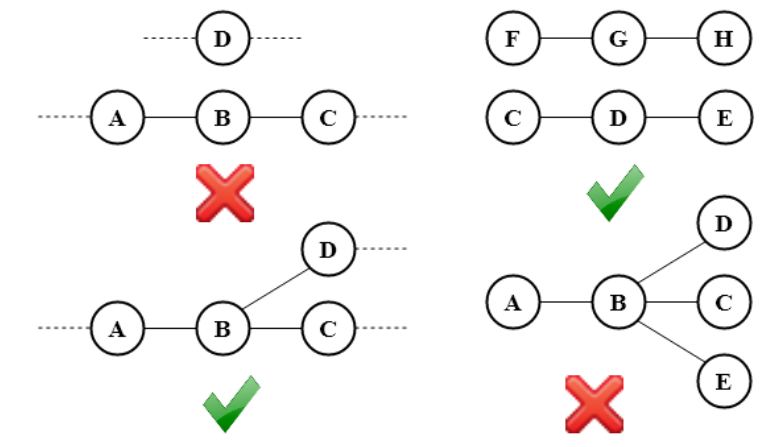
\includegraphics[width=1\textwidth]{Figuras/conexo.PNG}
        \centering\caption{Distintos tipos de redes de grafos.}
        \label{fig:conexidad}
    \end{figure}

    Para determinar si la red es conexa, se siguen los pasos del Algoritmo \ref{alg:connectedness}. Añadiendo nodos a una lista de zonas siempre que el nodo tenga un vecino en esa lista. Si un nodo posee un vecino en ambas listas, las listas se combinan, creando una nueva zona. Si la cantidad de zonas es uno entonces la red es fuertemente conexa. Una red ferroviaria disconexa puede resolverse mas rápido que una fuertemente conexa ya que no haría falta iterar entre todos los elementos para analizarlos sino solo los pertenecientes a dicho subgrafo.
        
    \begin{algorithm}\captionsetup{labelfont={sc,bf}, labelsep=newline}
        \label{alg:connectedness}
        \caption{Algoritmo de conexidad}
        \begin{algorithmic}
            \STATE \{zones\} $\gets \{ \}$
            \STATE ADD first node in \{zones\}
            \FOR {node in \{nodes\}}
                \FOR {zone in \{zones\}}
                    \IF {node not in zones[zone]}
                        \IF {neighbours(node) in zones[zone]}
                            \STATE zones[zone] ADD node
                        \ELSE
                            \STATE Define new\_zone
                            \STATE zones[new\_zone] ADD node
                        \ENDIF
                    \ENDIF
                \ENDFOR
            \ENDFOR 
            \OUTPUT \{zones\}   
        \end{algorithmic}
    \end{algorithm}
        
    En las siguientes subsecciones se analizaran en conjunto los elementos ferroviario descriptos en las clases FunctionalInfrastructure y InfrastructureVisualizations.
    
     % ELEMENTOS
    \subsection{Vías}
	\label{sec:tracks}
	
    Las vías férreas son el elemento ferroviario mas esencial, son la columna vertebral de la infraestructura ferroviaria. Estas constituyen el sitio por el cual se desplazan los trenes, definiendo no solo la dirección del desplazamiento, sino también restringiendo el dominio del tren. Esto lo diferencia de otros medios de transporte como el automóvil que, aún teniendo una carretera, puede moverse por fuera de esta.

    Las vías se encuentran separadas por una distancia fija que se mide desde sus caras internas, denominada trocha (Figura \ref{fig:vias_1}). Solamente las formaciones compatibles con ese parámetro de trocha pueden circular por el tendido ferroviario. El valor de la trocha puede variar entre las denominadas trocha angosta (600 a 1372 mm, estándar imperial británico) y trocha ancha (1520 a 2140 mm, estándar ruso, indio, ibérico, irlandés). Se estableció el valor intermedio de 1435 mm como valor de trocha internacional, usado ampliamente en Europa, Norteamérica y Oceanía.

    \begin{figure}[H]
        \centering
        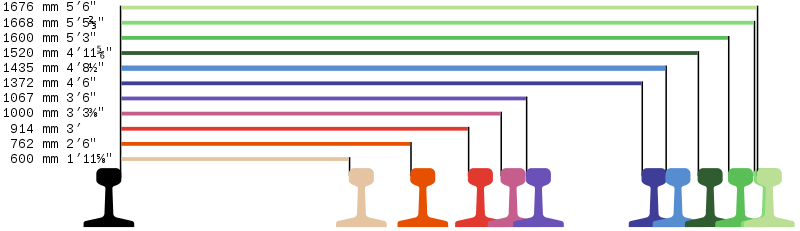
\includegraphics[width=1\textwidth]{Figuras/trocha.png}
        \centering\caption{Vías ferroviarias y trocha.}
        \label{fig:vias_1}
    \end{figure}
    
    Existen limitaciones logísticas y físicas por las cuales el tendido ferroviario no puede ser un continuo rígido. En primer lugar, las vías deben ser de un tamaño acotado, tal que puedan transportarse a la locación donde serán instaladas en tramos rectos o curvos. En segundo lugar, la dilatación y contracción de las vías debido a los cambios de temperatura añaden una restricción respecto a la distancia mínima que deben tener entre las mismas. De lo contrario, la dilatación del material puede provocar daños irreparables a la infraestructura y estos, a su vez, ser motivo de descarrilamientos, como ya ha ocurrido en los comienzos de la industria ferroviaria \cite{ACCIDENTE}. 
    
    Cada vía puede ser clasificada en dos grupos: vías ascendentes o vías descendentes (ver Figura \ref{fig:vias_2}). Las ascendentes son aquellas por las cuales los trenes circulan únicamente en la dirección del kilometraje en sentido creciente. Las descendentes son aquellas por las cuales los trenes circulan únicamente en la dirección del kilometraje en sentido decreciente \cite{RITO}. 

    \begin{figure}[H]
        \centering
        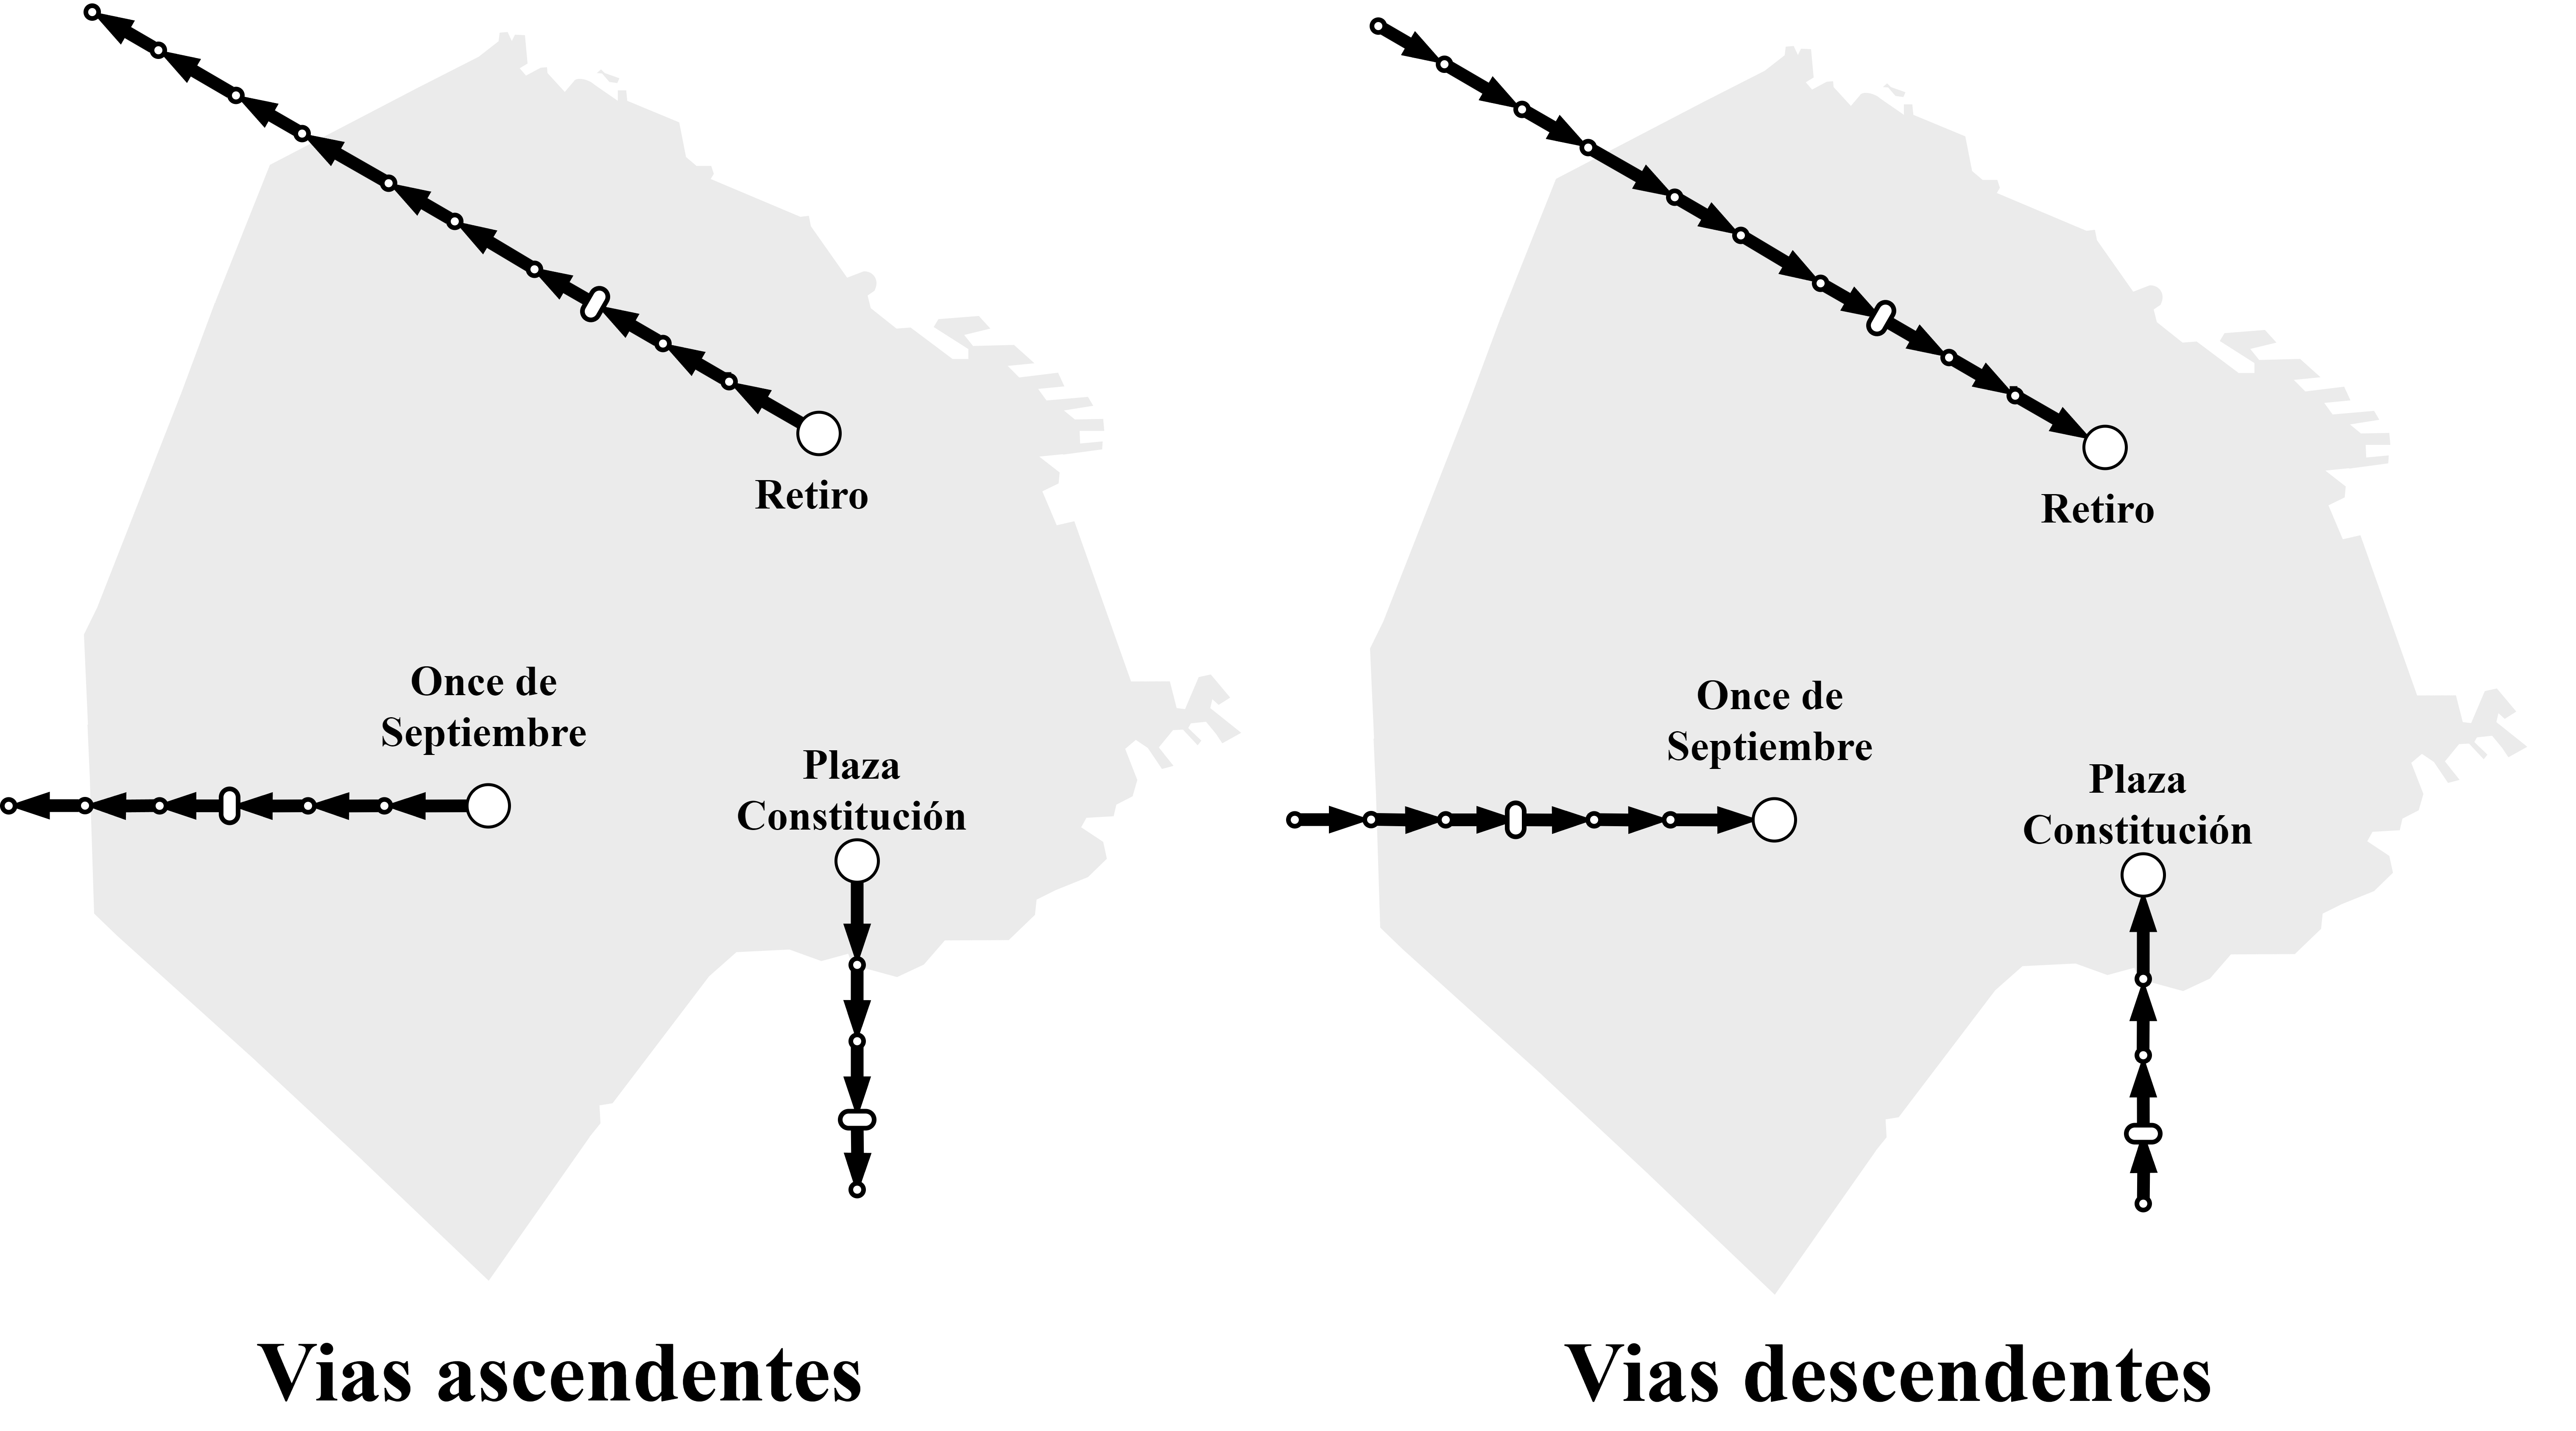
\includegraphics[width=1\textwidth]{Figuras/ascDesc.png}
        \centering\caption{Vías ascendentes y descendentes.}
        \label{fig:vias_2}
    \end{figure}

    El kilómetro cero es la estación principal de la línea ferroviaria, como pueden ser las terminales de Plaza Constitución (para la línea Roca), Once de septiembre (para la línea Sarmiento) y Retiro (para las líneas Mitre y San Martín).  Existen vías de maniobra que pueden ser tanto ascendentes como descendentes. Estas vinculan, mediante un cambio de vías, una sección ascendente con otra descendente, en la cual los trenes deben circular a una velocidad reducida. 

    Las vías se agrupan en secciones que, por cuestiones de seguridad y logística, se establece que solo pueden ser utilizadas por un tren a la vez. Estas secciones pueden ser de varios kilómetros en zonas rurales o unos pocos cientos de metros en zonas urbanas, donde la red necesita una mayor granularidad debido a la densidad del tráfico ferroviario en las grandes urbes.

    En railML las vías son elementos ferroviarios físicos, representados por la clase \textit{track}, ilustrada en el Código \ref{lst:track}. Esta clase se encuentra definida dentro del vector de clases \textit{tracks}, dentro de la clase \textit{functionalInfrastructure}, dentro de la clase \textit{infrastructure}.

    \begin{lstlisting}[language = XML, caption = Clase \textit{Track} , label = {lst:track}]
    <track type="mainTrack" infrastructureManagerRef="im_01" mainDirection="both" id="trk2">
        <trackBegin ref="bus5"/>
        <trackEnd ref="swi77"/>
        <length value="1799.28" type="physical"/>
        <designator register="Example" entry="TRACK track2"/>
        <linearLocation applicationDirection="both" id="trk2_lloc01">
            <associatedNetElement netElementRef="ne3" keepsOrientation="true"/>
        </linearLocation>
        <name name="track2" language="en"/>
    </track>
    \end{lstlisting}
    
    Las vías en railML se definen entre dos elementos ferroviarios físicos. En este caso, la vía indicada como trk2 se encuentra definida entre el \textit{BufferStop} bus5 (ver Sección \ref{sec:bufferstop}) y el cambio de vías swi77 (ver Sección \ref{sec:switches}). Esta clase define, además, el largo de la vía y el \textit{netElement} al cual están asociadas, en este caso, el \textit{netElement} ne3. Es natural confundirse \textit{tracks} y \textit{netElements}, porque son términos casi equivalentes, pero un track representa un elemento físico y un \textit{netElement} engloba de manera abstracta una porción del trazado de vías. Es decir, una vía puede dividirse en varios \textit{netElements}, pero un \textit{netElement} solo se asocia a una vía.
    \subsection{Fin de vía y transiciones}
    \label{sec:bufferstop}

    El tendido ferroviario no puede continuar de forma indefinida, ni tampoco interrumpirse de forma abrupta. Como se puede visualizar en la Figura \ref{fig:frontera_1}, existen dos formas de definir el fin de vía: de forma relativa y de forma absoluta.

    \begin{figure}[H]
        \centering
        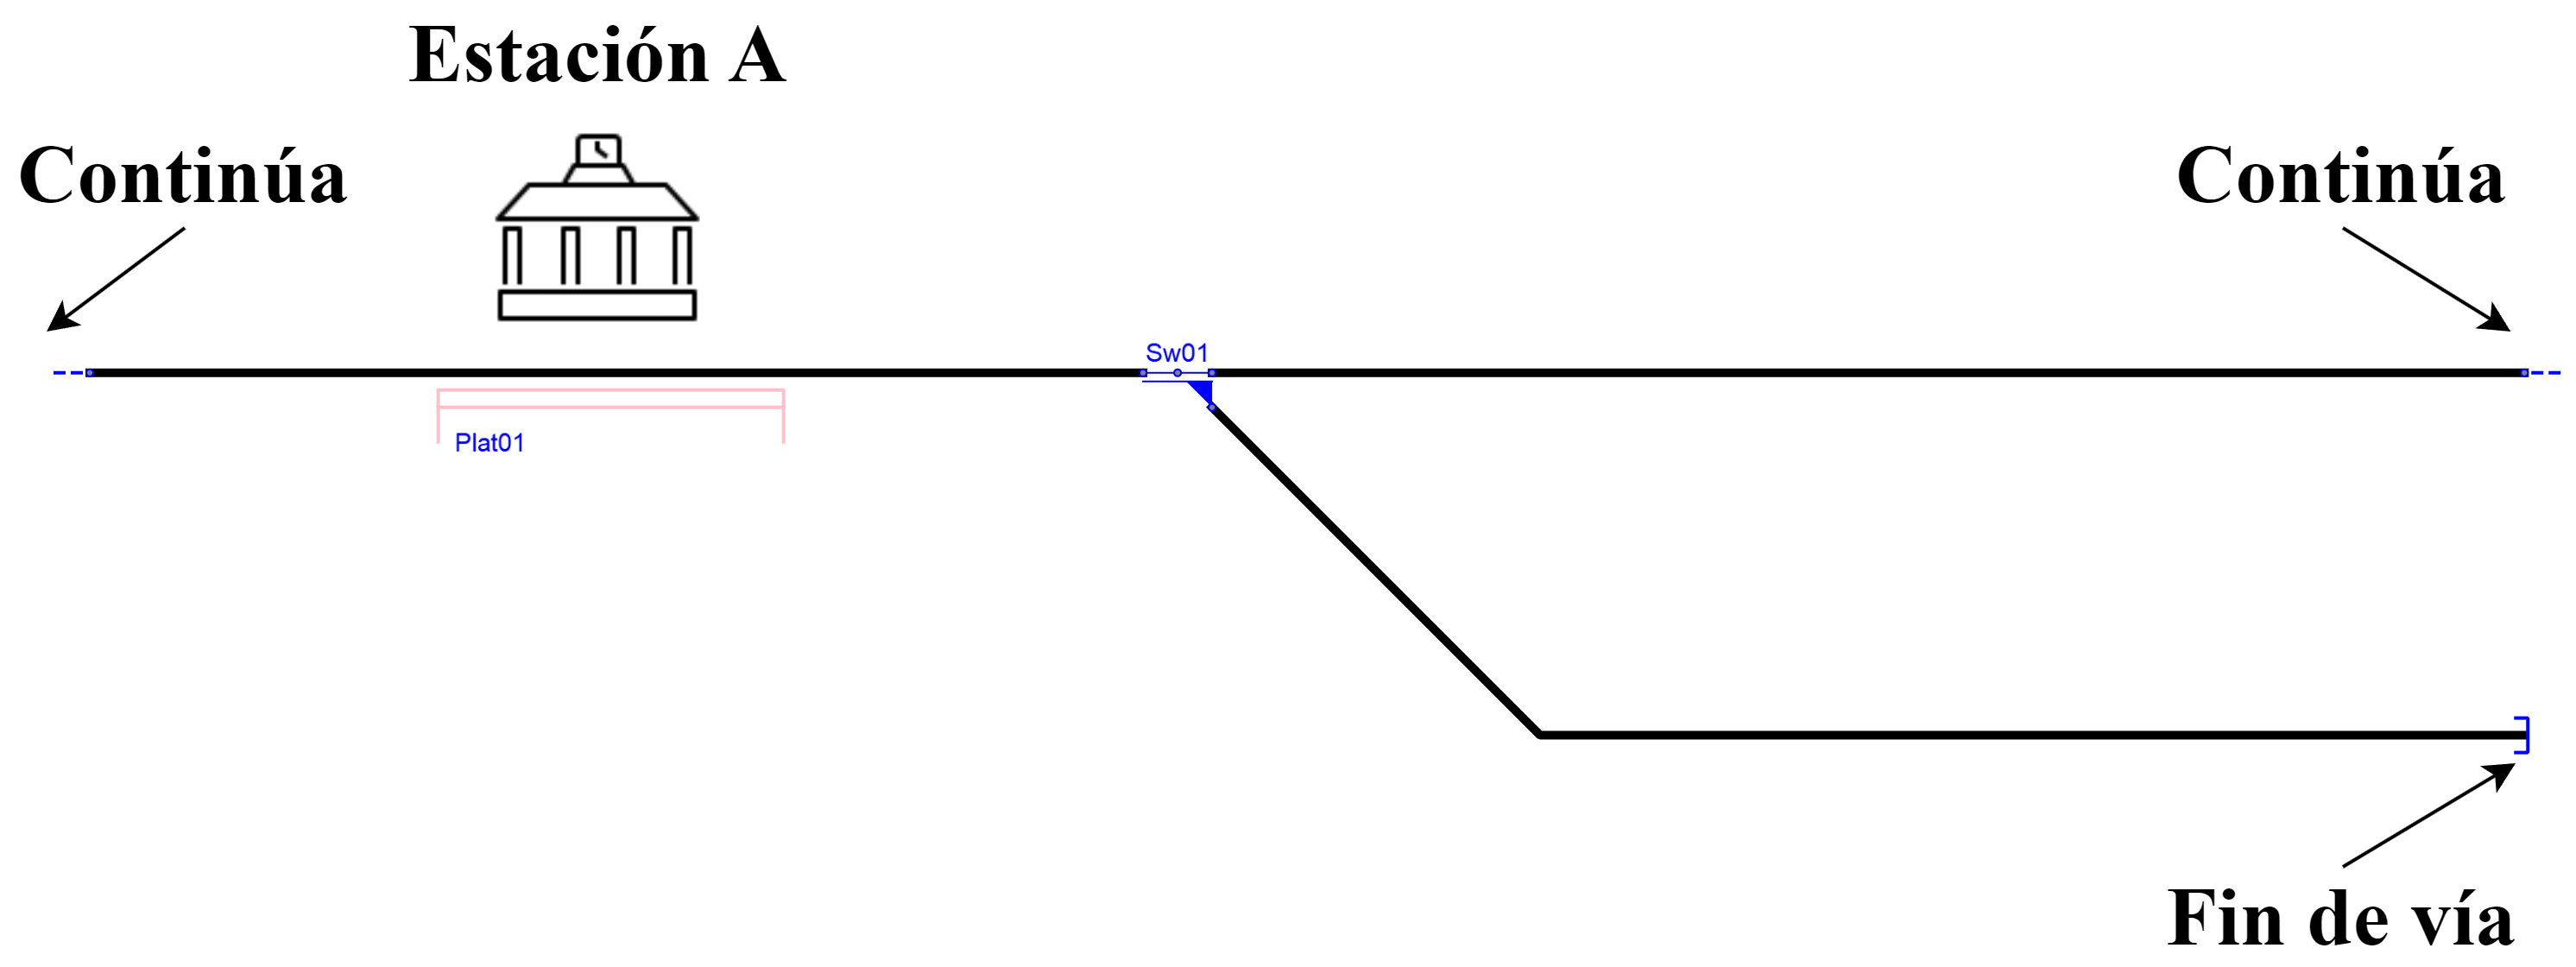
\includegraphics[width=0.9\textwidth]{Figuras/Border.png}
        \centering\caption{Topología de ejemplo con finales de vía relativos y absolutos.}
        \label{fig:frontera_1}
    \end{figure}

    Un ejemplo de fin de vía relativo sería la frontera entre las estaciones A y B. Las vías continúan a la derecha de A, pero no son parte del alcance del sistema que controla los elementos ferroviarios en las inmediaciones de A. En tanto que un fin de vía absoluto sería todo final literal de la red ferroviaria, tales como terminales, talleres y vías secundarias sin retorno, como la ramificación saliente de la vía principal.
    
    Un fin de vía relativo es todo aquel límite que define el alcance del sistema de señalamiento, pero no necesariamente es el final de la red. Es decir, el sistema podrá recibir información de cualquier sensor dentro de estos límites, o incluso de algunos sensores en la frontera exterior, pero solo podrá comandar los actuadores dentro de la zona. Esto es de vital importancia a la hora de reducir la complejidad de la red, al realizar el procesamiento de forma distribuida, sin depender de un decisión centralizada.

    Este elemento ferroviario es modelo por la clase border, cuyo ejemplo se visualiza en el Código \ref{lst:lineBorder}. Siempre se definen referido a un único netElement, en este caso el netElement ne114 y a una coordenada intrínseca que puede ser 0 si se encuentra al principio del netElement, o de 1 si se encuentra al final.

    \begin{lstlisting}[language = XML, caption = Clase border , label = {lst:lineBorder}]
    <border isOpenEnd="false" externalRef="" type="station" id="sb540">
        <designator register="_Example" entry="BORDER SB05"/>
        <spotLocation netElementRef="ne114" intrinsicCoord="0.0000" applicationDirection="reverse" id="sb540_sloc01"/>
        <name name="SB05" language="en"/>
    </border>
    \end{lstlisting}

    Un fin de vía absoluto es todo aquel límite que define el final físico del tendido ferroviario, luego del cual ya no se tiene infraestructura. Podemos encontrar estos límites en los talleres ferroviarios, en las terminales principales de cada red o en vías utilizadas para estacionar los trenes por fuera de la rama principal en uso. Estos límites deben estar adecuadamente protegidos y señalizados.

    Este elemento ferroviario es modelo por la clase bufferStop, cuyo ejemplo se visualiza en el Código \ref{lst:bufferStop}. Al igual que la clase border, se definen referido a un único netElement, en este caso el netElement ne3 y a una coordenada intrínseca que puede ser 0 si se encuentra al principio del netElement, o de 1 si se encuentra al final.
    
    \begin{lstlisting}[language = XML, caption = Clase bufferStop , label = {lst:bufferStop}]
    <bufferStop type="fixedBufferStop" id="bus5">
        <designator register="_Example" entry="BUFFERSTOP Buf05"/>
        <spotLocation netElementRef="ne3" intrinsicCoord="0.0000" applicationDirection="reverse" id="bus5_sloc01"/>
        <name name="Buf05" language="en"/>
    </bufferStop>
    \end{lstlisting}
    \subsection{Sistemas de detección de formaciones ferroviarias}
    \label{sec:detectors}
    
    Es de vital importancia que el sistema pueda determinar la posición de un tren dentro del tendido ferroviario. De esta manera, poder habilitar la circulación en secciones donde no exista peligro de colisión con otros formaciones o, por el contrario, detener la marcha de las formaciones anteriores para evitar accidentes. Existen diversas maneras de detectar la posición de un tren, entre ellas el uso de circuitos de vía y contadores de ejes (Figura \ref{fig:deteccion_1}). 

    \begin{figure}[H]
        \centering
        \includegraphics[width=1\textwidth]{Figuras/detector}
        \centering\caption{Circuito de vía (01) y contador de ejes (AxC01).}
        \label{fig:deteccion_1}
    \end{figure}

    Los circuitos de vía (Figura \ref{fig:deteccion_2}) son dispositivos eléctricos que aplican una diferencia de potencial entre los rieles. Cuando una formación ingresa a la sección, sus ruedas metálicas cortocircuitan ambos rieles. El cortocircuito es detectado por el relé, que a su vez, reporta el estado al resto del sistema. 

    \begin{figure}[H]
        \centering
        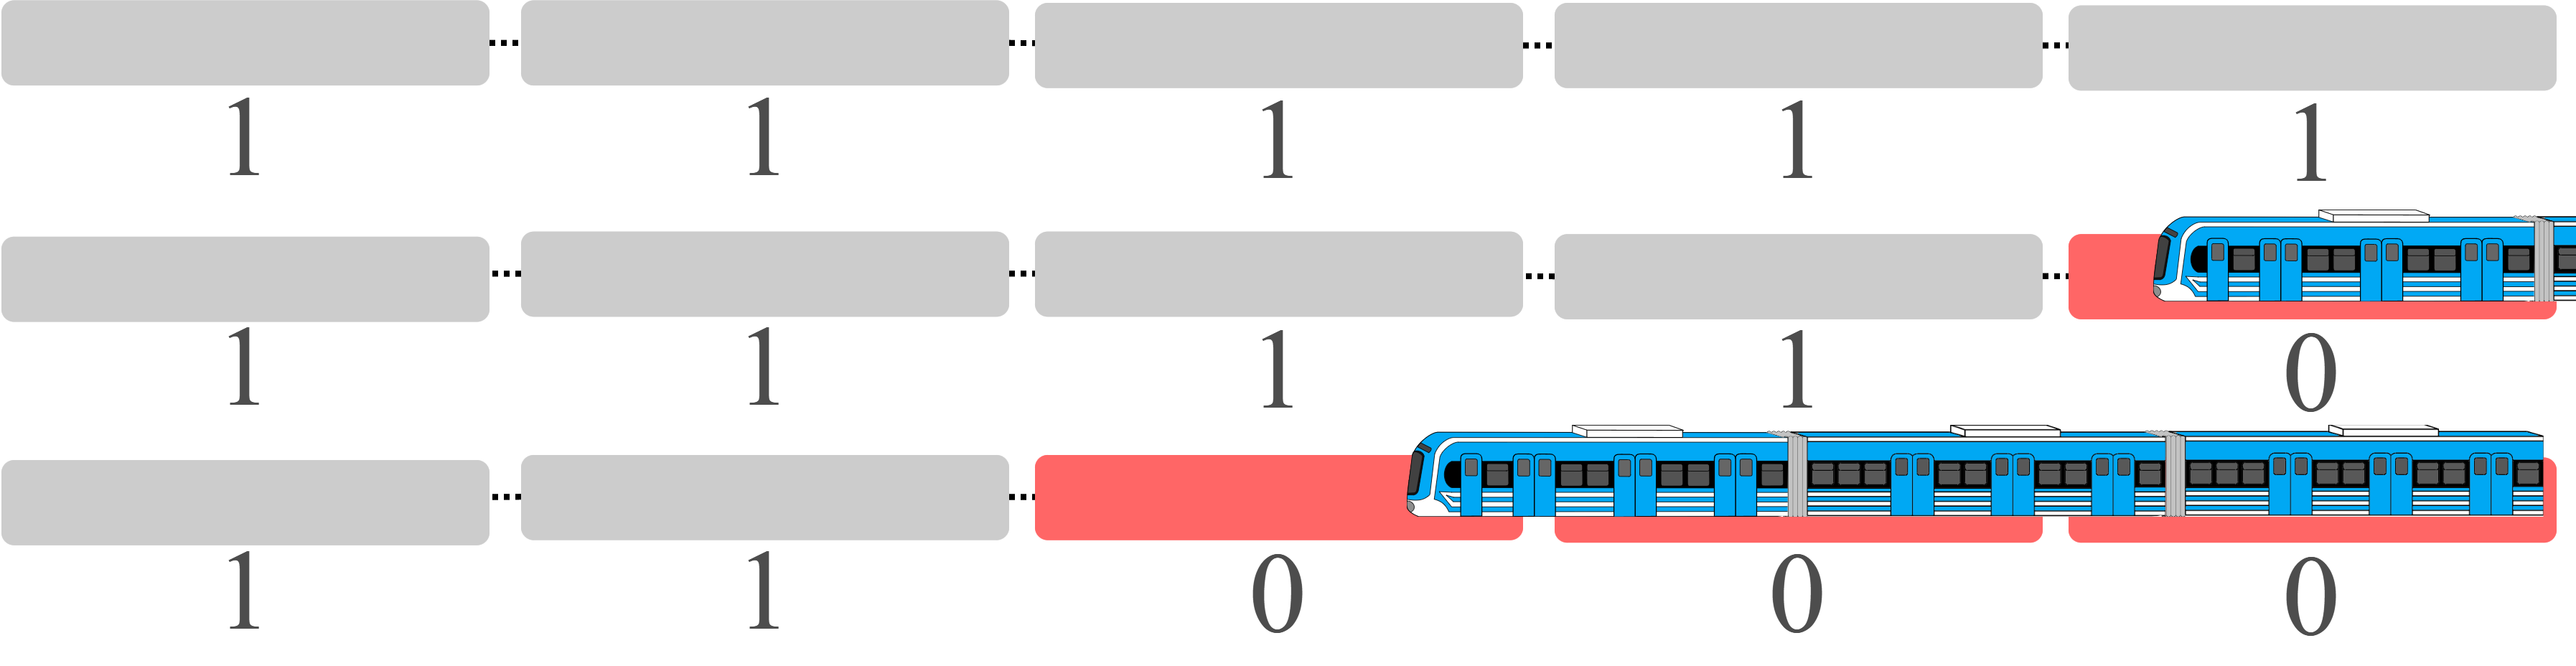
\includegraphics[width=1\textwidth]{Figuras/circuitoVia}
        \centering\caption{Circuito de vía libre y ocupado.}
        \label{fig:deteccion_2}
    \end{figure}

    En caso de que la alimentación se interrumpa, el cableado sufra alguna falla, vandalismo, inundación, o que efectivamente una formación ocupe la sección, el circuito de vía reportará que la sección se encuentra ocupada. De esta manera, solo es posible recibir un reporte de sección desocupada cuando la sección efectivamente se encuentre desocupada. A este principio se le denomina fail-safe \cite{Paper_5,Paper_94,Paper_95,Paper_96}. Es decir, si por alguna razón algo falla, el sistema adopta la condición más restrictiva, mitigando la posibilidad de una situación peligrosa. 
    
    Existe una discontinuidad entre los rieles denominado juntura, que permite la expansión de los mismos al ser sometidos a altas temperaturas sin que los rieles se doblen y provoquen daños a la infraestructura. Los circuitos de vía, se relacionan directamente a las junturas entre las vías, modelados por la clase \textit{railJoint} en railML.  Esta discontinuidad eléctrica es lo que limita la acción del circuito de vía a la región entre dos junturas.

    En el código \ref{lst:trackCircuit} podemos ver un ejemplo de la clase \textit{tvdSection} dentro de la clase \textit{interlocking}, que incluye a la clase \textit{assetsForIL} y estos, a su vez, a la clase vector de \textit{tvdSections}. Esta clase posee un id (tvd7), la tecnología utilizada (en este caso \textit{trackCircuit}, circuito de vía) y los límites donde el circuito de vía es válido: los \textit{bufferStop} bus1 y bus2.

    \begin{lstlisting}[language = XML, caption = Clase \textit{TrackCircuit} , label = {lst:trackCircuit}]
    <tvdSection id="tvd7" partialRouteReleaseDelay="PT4S" residualRouteCancellationDelay="PT90S" technology="trackCircuit" isBerthingTrack="false">
        <designator register="Example" entry="01"/>
        <hasDemarcatingBufferstop ref="bus2"/>
        <hasDemarcatingBufferstop ref="bus1"/>
    </tvdSection>
    \end{lstlisting}

    Los sistemas contadores de ejes (Figura \ref{fig:deteccion_2}) consisten en sensores pasivos instalados en la cara interna de unos de los rieles y un sistema externo de procesamiento de datos. Estos sistemas no dependen de la aplicación de tensiones en la vía. Además, no solo permiten detectar la presencia de una formación, sino que también pueden usarse para medir la integridad de la formación, si se conoce a priori la cantidad de ejes de la misma. 

    \begin{figure}[H]
        \centering
        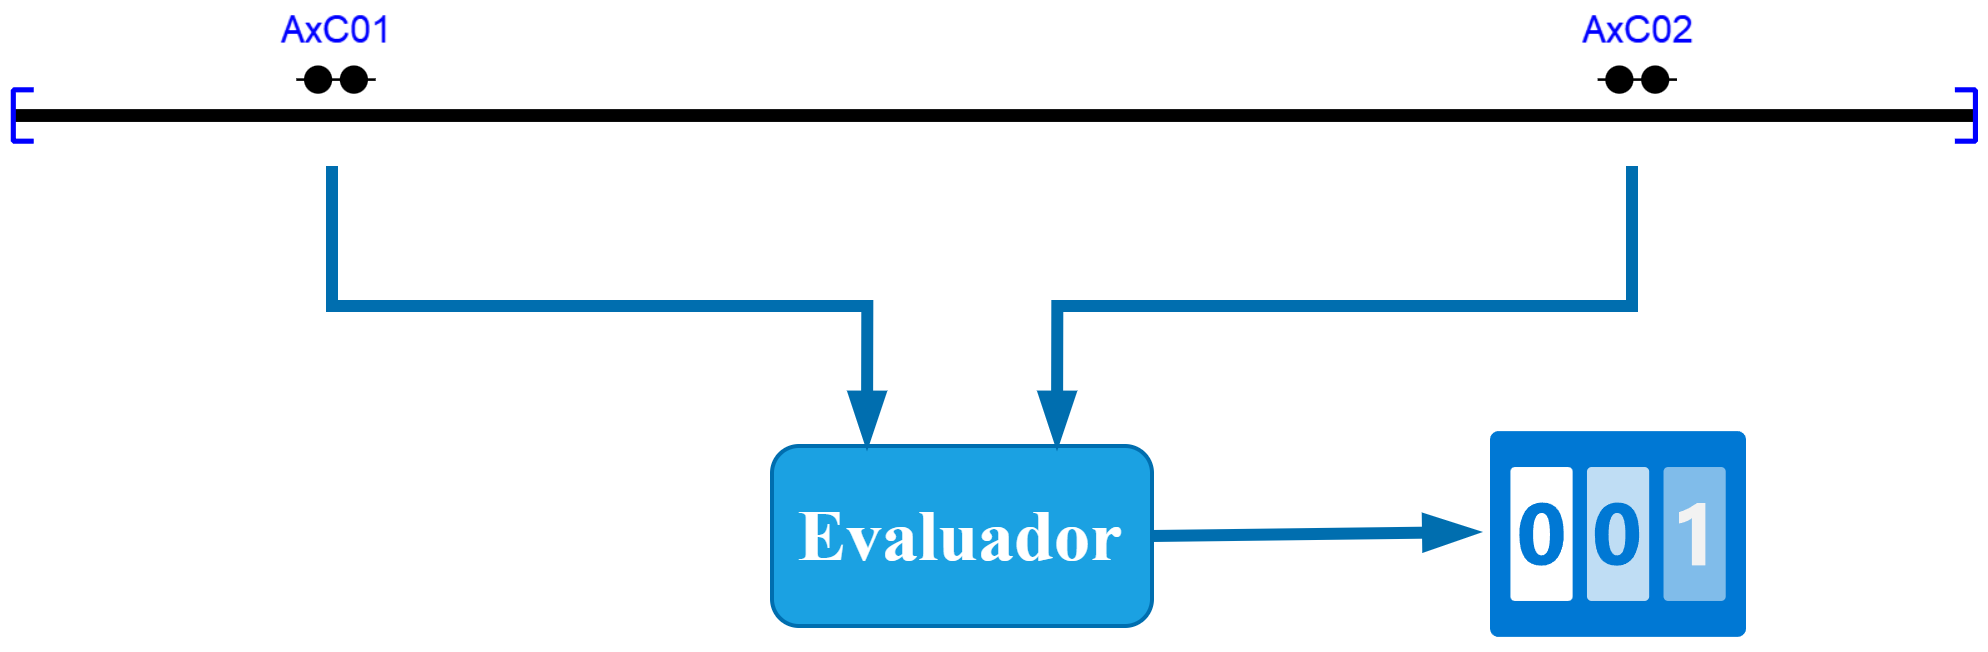
\includegraphics[width=1\textwidth]{Figuras/contador}
        \centering\caption{Contadores de ejes.}
        \label{fig:deteccion_2}
    \end{figure}

    Al igual que los circuitos de vía, los sistemas contadores de eje siguen el principio de fail-safe, adoptando la condición mas restrictiva en caso de falla. Ambos sistemas pueden utilizarse en simultáneo, de ser requerido. En el código \ref{lst:axleCounter} podemos ver un ejemplo de la clase \textit{trainDetectionElement}, dentro de la clase \textit{functionalInfrastructure}, dentro de la clase \textit{infrastructure}. En este ejemplo la bclase fue definida como tipo \textit{axleCounter} (contador de eje) y se le asigna el nombre AxC01 que vemos en la Figura \ref{fig:deteccion_1}, referido al \textit{netElement} ne1. También podemos ver que este contador de ejes se activa en ambos sentidos (applicationDirection = both) y su coordenada intrínseca dentro del \textit{netElement} ne1, dentro de los dos tercios de la sección.

    \begin{lstlisting}[language = XML, caption = Clase \textit{TrainDetectionElement} , label = {lst:axleCounter}]
    <trainDetectionElement id="ac6" type="axleCounter">
        <name name="AxC01" language="en"/>
        <spotLocation id="ac6_sloc01" netElementRef="ne1" applicationDirection="both" intrinsicCoord="0.6710"/>
        <designator register="Example" entry="TRAIN DETECTION ELEMENT AxC01"/>
    </trainDetectionElement>
    \end{lstlisting}
    \subsection{Automatic Train Stop (ATS)}

\lipsum[1]

    \begin{figure}[!h]
        \centering
        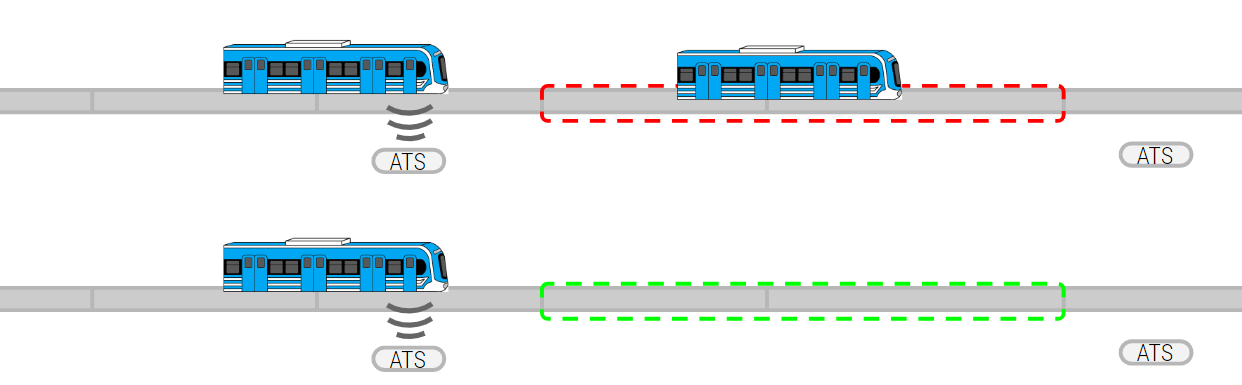
\includegraphics[width=1\textwidth]{Figuras/ATS}
        \centering\caption{ATS.}
        \label{fig:ATS_1}
    \end{figure}

\lipsum[1]
    \subsection{Estaciones ferroviarias}
    \label{sec:platform}
    
    Las estaciones ferroviarias son las zonas donde las formaciones pueden detenerse para que los pasajeros puedan descender y nuevos pasajeros puedan abordar. En función del tamaño de las formaciones y la geografía del lugar, las plataformas desde donde ascienden y descienden los pasajeros pueden estar elevadas con respecto al suelo o a ras del mismo. El largo de las plataformas también depende de la cantidad de coches de las formaciones.
    
    Como puede verse en la Figura \ref{fig:estacion_1}, las estaciones ferroviarias incluyen no solo a las plataformas, sino que también pueden centralizar el control de varias operaciones logísticas como la asignación de rutas. No obstante, en este trabajo nos referiremos a las estaciones como plataformas indistintamente.
    
        \begin{figure}[H]
            \centering
            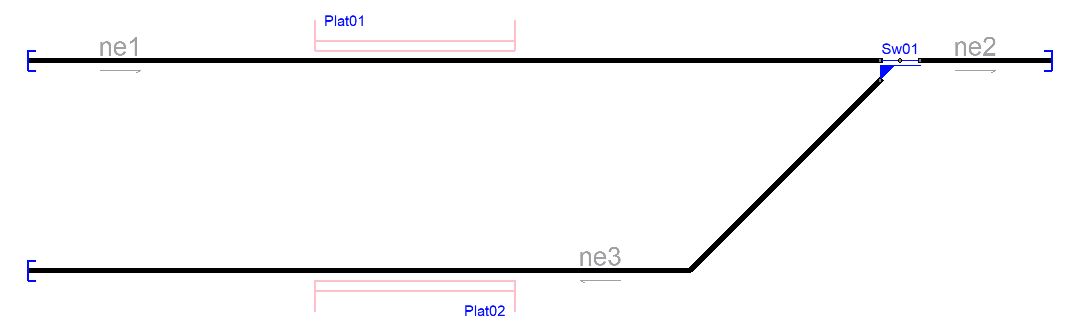
\includegraphics[width=1\textwidth]{Figuras/Platform.png}
            \centering\caption{Estación de doble plataforma.}
            \label{fig:estacion_1}
        \end{figure}
    
    Las estaciones de mayor complejidad o de mayor convergencia de ramales suelen concentrar el control de la estación donde se encuentran y varias estaciones vecinas. Las estaciones terminales, a menudo, pueden incluso tener control total de varios ramales completos.

    En el Código \ref{lst:platform_1} se pueden ver la implementación de la clase platform de las plataformas ilustradas en la Figura \ref{fig:estacion_1}. Esta clase se encuentra dentro de la clase infrastructure, que a su vez contiene a la clase functionalInfrastructure. La misma incluye atributos como la altura, el nombre asignado que se visualiza en la Figura \ref{fig:estacion_1} y el netElement al que se encuentran asociadas cada una de las plataformas.

    \begin{lstlisting}[language = XML, caption = Clase Platform , label = {lst:platform_1}]
    <platforms>
        <platform id="plf3" height="0">
            <name name="Plat01" language="en"/>
            <linearLocation id="plf3_lloc01" applicationDirection="both">
                <associatedNetElement keepsOrientation="true" netElementRef="ne1"/>
            </linearLocation>
            <designator register="_Example" entry="PLATFORM Plat01"/>
            <length type="physical" value="0" validForDirection="both"/>
        </platform>
        <platform id="plf6" height="0">
            <name name="Plat02" language="en"/>
            <linearLocation id="plf6_lloc01" applicationDirection="both">
                <associatedNetElement keepsOrientation="true" netElementRef="ne3"/>
            </linearLocation>
            <designator register="_Example" entry="PLATFORM Plat02"/>
            <length type="physical" value="0" validForDirection="both"/>
        </platform>
    </platforms>
    \end{lstlisting}

    Los datos relativos a la características físicas como el largo y el ancho la encontramos dentro de la clase visualization, dentro de la clase infrastructureVisualizations, como se puede ver en el Código \ref{lst:platform_2}.

    \begin{lstlisting}[language = XML, caption = Clase visualization , label = {lst:platform_2}]
    <spotElementProjection refersToElement="plf3" id="vis01_sep4">
        <name name="Plat01" language="en"/>
        <coordinate x="-125.455" y="-240.000"/>
    </spotElementProjection>
    <spotElementProjection refersToElement="plf6" id="vis01_sep5">
        <name name="Plat02" language="en"/>
        <coordinate x="-125.454" y="-30.000"/>
    </spotElementProjection>
    \end{lstlisting}

    Conocer las dimensiones del elemento físico que representa esta clase es fundamental a la hora de analizar el impacto de este elemento en la red y donde se deberían asignar las señales ferroviarias.
    \subsection{Cruces ferroviarios}

Los cruces ferroviarios son la intersección entre la vía ferroviaria y una ruta vehicular o peatonal. Estos cruces pueden ser bajo nivel (túnel por debajo de la vía), sobre nivel (puente vehicular por sobre la vía) o a nivel. Un paso a nivel es una zona muy crítica del sistema ferroviario, ya que, a diferencia de un paso sobre nivel o bajo nivel, conviven simultáneamente la formación y el transito vehicular y peatonal. En la Figura \ref{fig:cruce_1} se ilustra la intersección entre el tendido ferroviario, un cruce vehicular y un cruce peatonal.

    \begin{figure}[!h]
        \centering
        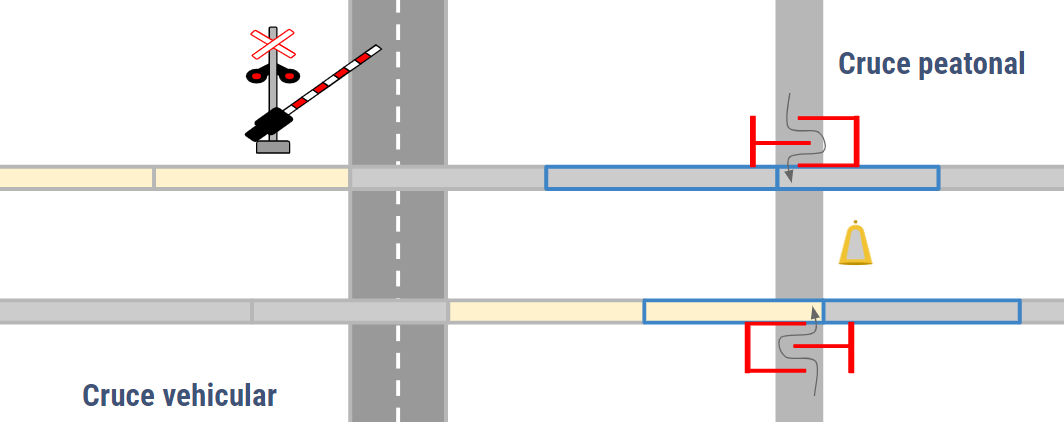
\includegraphics[width=1\textwidth]{Figuras/cruce}
        \centering\caption{XXXXX.}
        \label{fig:cruce_1}
    \end{figure}
    
Los pasos a nivel peatonales incluyen un pequeño laberinto zigzagueante para forzar al peatón a aminorar su marcha y ver a ambos lados antes de cruzar las vías. A menudo suelen estar acompañados de indicaciones lumínicas y sonoras que se accionan tan pronto el tren se encuentre dentro de un rango de varios metros cercano al paso a nivel.

Los pasos a nivel vehiculares añaden barreras ferroviarias para detener el tráfico vehicular cuando un tren se encuentra dentro de un rango de seguridad definido.  El sistema de control de la barrera mantiene el brazo de esta en alto para permitir la circulación vehicular. Si un tren es detectado cerca del paso a nivel, se desenergiza la barrera y comienza a descender el brazo por efecto de la gravedad. Solo cuando la barrera baja, el tren tiene permitido avanzar sobre el cruce, siendo el paso a nivel un sector de altísimo riesgo. Al desocuparse las secciones próximas al paso a nivel, la barrera vuelve a energizarse y se sitúa en estado alto nuevamente, a la espera de otro tren para reiniciar el proceso. 

Se debe destacar que el mismo proceso de descenso de la barrera ocurrirá si esta se desenergiza por una falla electricomecánica y/o pérdida de alimentación. Es decir, el sistema asumirá el estado más seguro ante cualquiera de los mencionados fallos, siguiendo el principio de falla segura.
    \subsection{Máquina de cambios}
    \label{sec:switches}
 
    Una máquina de cambios (Figura \ref{fig:cambios_1}) es un mecanismo utilizado para permitir el paso de las formaciones de una vía a una ramificación del recorrido principal. Esto se realiza mediante el movimiento de la aguja del cambio (riel móvil) hacia su respectiva contraaguja (riel fijo) hasta obtener un adecuado acoplamiento que permita la circulación de la formación.

    \begin{figure}[!h]
        \centering
        \includegraphics[width=0.9\textwidth]{Figuras/Cambios.jpg}
        \centering\caption{Máquina de cambios.}
        \label{fig:cambios_1}
    \end{figure}

    En la Figura \ref{fig:cambios_2} se muestra el cambio de vía de la estación Matheu de la Línea Mitre. Se observa que según sea la posición de la máquina de cambios, el tren puede continuar en la misma vía o hacer el cambio a la otra vía.

    \begin{figure}[!h]
        \centering
        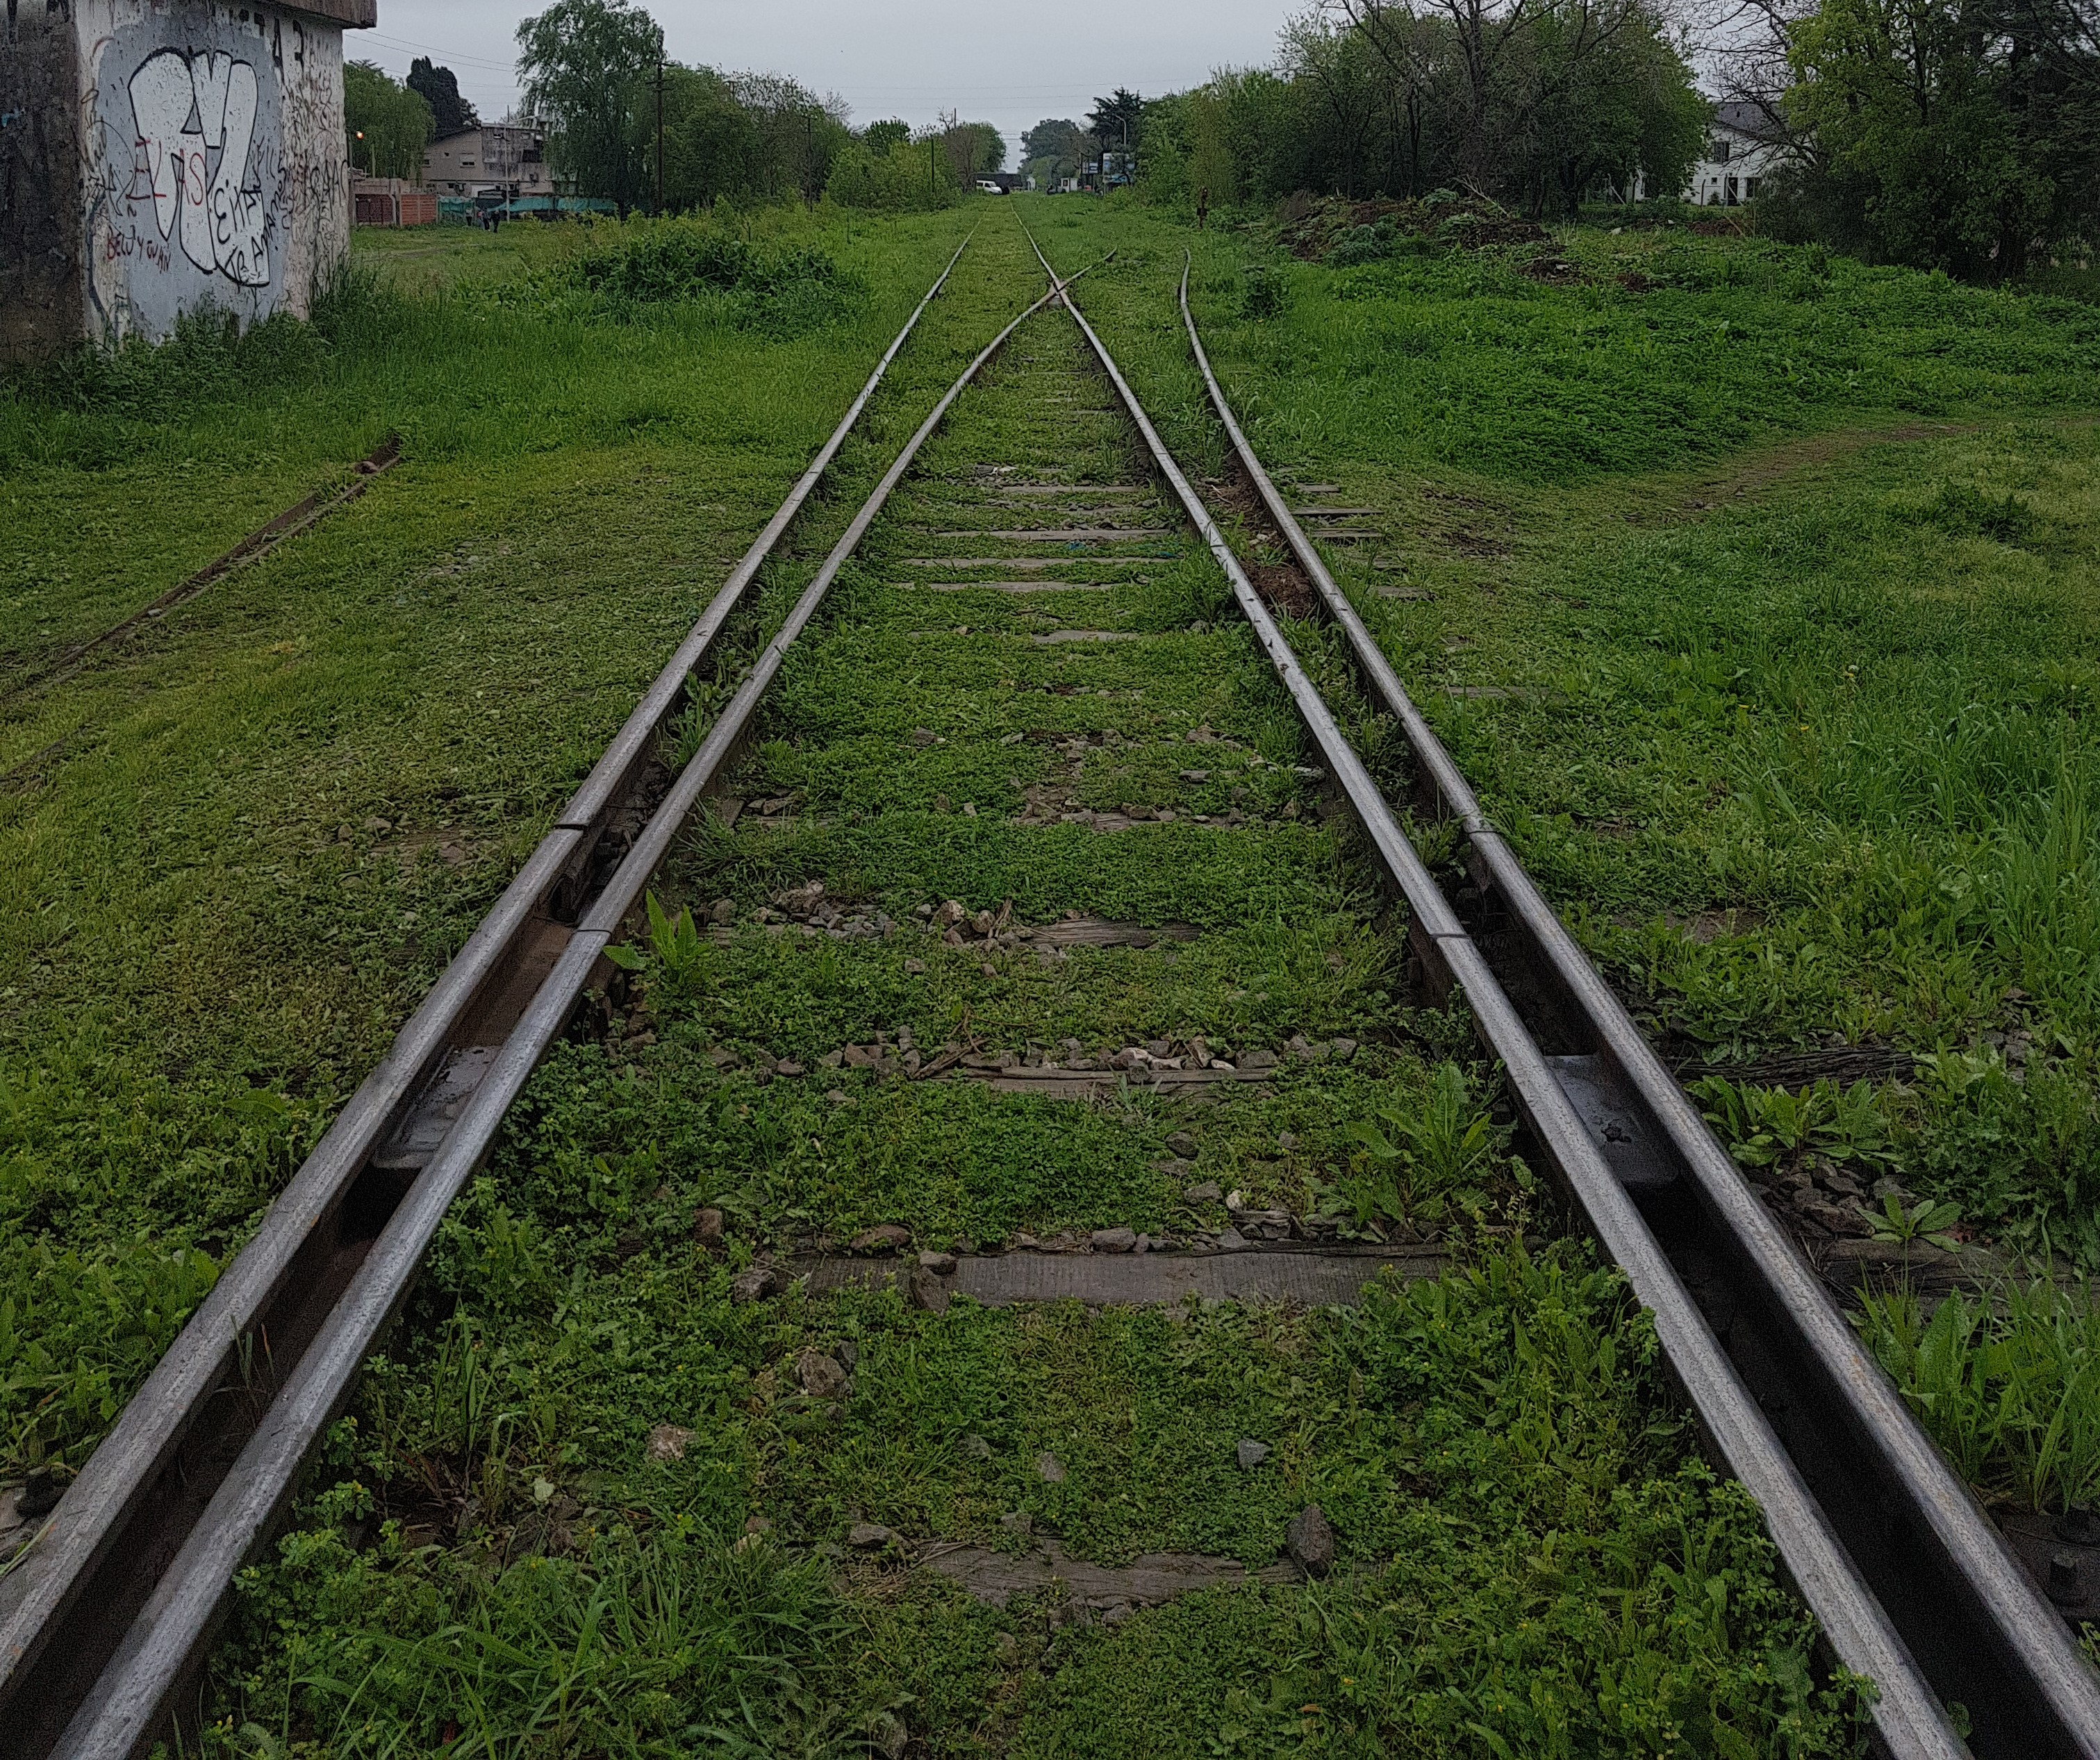
\includegraphics[width=0.9\textwidth]{Figuras/Cambios_2.jpg}
        \centering\caption{Cambio de vías de estación Matheu, Linea Mitre.}
        \label{fig:cambios_2}
    \end{figure}

    En la Figura \ref{fig:cambios_3} se muestran las posiciones que puede adoptar el cambio. En la posición normal, los trenes pueden circular de forma directa, en paralelo, por la vía principal en sentidos opuestos. En la posición reversa, en cambio, se permite el intercambio de trenes de una rama principal a otra en sentido opuesto o a una ramificación secundaria de la red.

    \begin{figure}[!h]
        \centering
        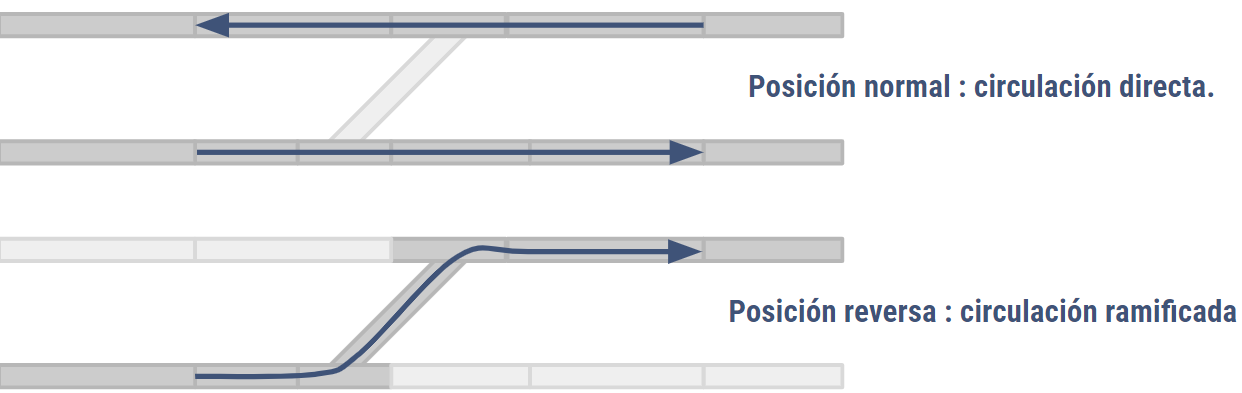
\includegraphics[width=0.9\textwidth]{Figuras/cambio_3.PNG}
        \centering\caption{Posiciones adoptadas por una máquina de cambios simple.}
        \label{fig:cambios_3}
    \end{figure}

    Las máquinas de cambios son un elemento activo de la red ferroviaria, controlados por el sistema de enclavamientos. Al ser mecanismos que necesitan tiempo para cambiar de un estado al otro, no puede asumirse que el comando es obedecido al instante. Incluso podría darse el caso que jamás llegue a cumplirse la orden debido a desperfectos mecánicos o eléctricos. Es por eso que introducimos los conceptos de comando, indicación y correspondencia, tal como se ilustran en la Figura \ref{fig:cambios_4}.

    \begin{figure}[!h]
        \centering
        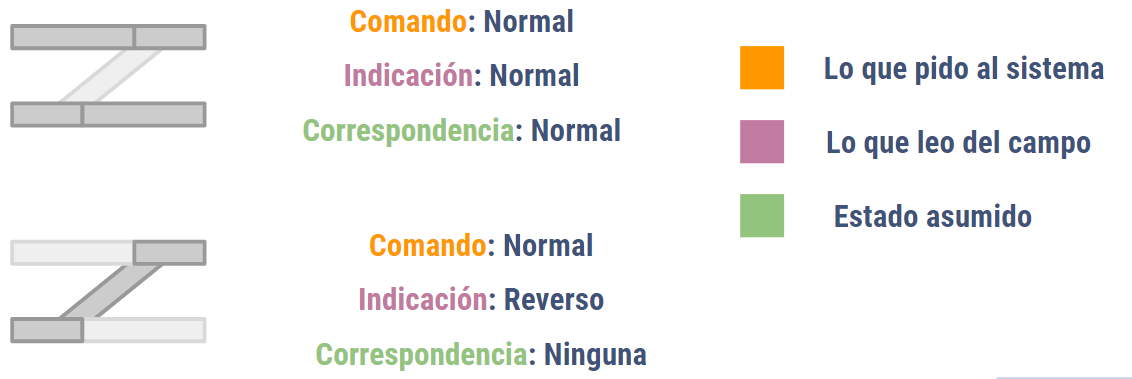
\includegraphics[width=1\textwidth]{Figuras/cambios}
        \centering\caption{Comando, indicación y correspondencia en máquinas de cambios.}
        \label{fig:cambios_4}
    \end{figure}
    
    El comando es la instrucción que el sistema de enclavamientos envía a la máquina de cambios. Esta instrucción puede ser modificar la posición de normal a reverso o de reverso a normal. La indicación es el estado que la máquina de cambios informa al sistema de enclavamientos. El sistema solo asume que el comando fue obedecido cuando tanto el comando como la indicación muestran una correspondencia. En caso contrario, el sistema de enclavamiento no puede asumir cual es el estado real del sistema, si el comando enviado o el estado reportado por la máquina de cambios. El mismo concepto puede ser aplicado en cualquier otro elemento mecánico, como por ejemplo las barreras ferroviarias.

    El RNA debe analizar diversos atributos distribuidos entre la clase switchIS (Código \ref{lst:switchIS}), la clase spotElementProjection (Código \ref{lst:switch}) y switchIL (Código \ref{lst:switchIL}). La clase switchIS se encuentra dentro del vector de clases switchesIS, dentro de functionalInfrastructure, que a su vez es parte de la clase infrastructure. La clase define el id de la máquina de cambios, el tipo (ordinario), el netElement al cual pertenece la entrada del cambio y hacia que lado se encuentra la vía de continuación y ramificación si transitamos desde el netElement del cambio hacia el cambio mismo. En este caso, si transitamos por el netElement ne16 el tren tendrá la vía de continuación en la mano derecha y la ramificación en la mano izquierda. Las máquina de cambio ordinarias siempre tienen una rama izquierda y una rama derecha definida. Además, dentro de la definición de cada rama tenemos el atributo netRelationRef, del cual se puede obtener, procesamiento mediante, los otros netElement correspondientes a las ramas: ne15 y ne14.

    \begin{lstlisting}[language = XML, caption = Clase switchIS , label = {lst:switchIS}]
    <switchIS id="swi84" continueCourse="right" branchCourse="left" type="ordinarySwitch">
        <name name="Sw01" language="en"/>
        <spotLocation id="swi84_sloc01" netElementRef="ne16" applicationDirection="reverse" intrinsicCoord="0.0000"/>
        <designator register="_Example" entry="SWITCH Sw01"/>
        <leftBranch netRelationRef="nr_ne15ne16_swi84" branchingSpeed="0" joiningSpeed="0" radius="-500"/>
        <rightBranch netRelationRef="nr_ne14ne16_swi84" branchingSpeed="0" joiningSpeed="0" radius="0"/>
    </switchIS>
    \end{lstlisting}

    La clase spotElementProjection define la ubicación en el espacio del elemento ferroviario referido. En este caso, como se puede ver en el Código \ref{lst:switch}, la posición de la máquina de cambios es la coordenada (-561 ; -450).

    \begin{lstlisting}[language = XML, caption = Clase spotElementProjection , label = {lst:switch}]
    <spotElementProjection refersToElement="swi84" id="vis01_sep16">
        <name name="Sw01" language="en"/>
        <coordinate x="-560.994" y="-450.000"/>
    </spotElementProjection>
    \end{lstlisting}

    La clase switchIL, definida dentro del vector de clases switchesIL, se encuentra dentro de la clase assetsForIL, en la clase interlocking. Contiene datos extra sobre el comportamiento dinámico de la máquina de cambios y define explícitamente los otros dos nodos, en contraposición a switchIS del cual hay que obtenerlos procesando un string. El RNA puede obtener los netElement de ambas clases y compararlos, anulando el análisis si los netElement definidos en switchIS y switchIL no son coincidentes.
    
    \begin{lstlisting}[language = XML, caption = Clase switchIL , label = {lst:switchIL}]
    <switchIL id="il_swi84" maxThrowTime="PT10S" typicalThrowTime="PT6S" isKeyLocked="false" returnsToPreferredPosition="false">
        <refersTo ref="swi84"/>
        <branchLeft ref="ne15"/>
        <branchRight ref="ne14"/>
    </switchIL>
    \end{lstlisting}
    
    El RNA utiliza el Algoritmo \ref{alg:switches} para detectar todos estos parámetros y crear un vector de máquinas de cambios (switches) indexado por el id de cada máquina de cambios (sw\_id). La existencia y ubicación de las máquinas de cambios ya se habían obtenido mediante el análisis de la red de grafos ferroviaria. El Algoritmo \ref{alg:switches} analiza la clase switchIS y confirma la existencia de la máquina de cambios, para luego la clase spotElementProjection y confirmar la ubicación de la misma. Los datos obtenidos en switches[sw\_id].LeftBranch y switches[sw\_id].RightBranch, permiten obtener los nodos de las ramificaciones que luego se conformarán analizando la clase switchIL en algoritmos posteriores.

    \begin{algorithm}\captionsetup{labelfont={sc,bf}, labelsep=newline}
            \caption{Algoritmo detector de máquinas de cambios.}
            \label{alg:switches}
            \begin{algorithmic}
                \STATE \{switches\} $\gets$ \{\}
                \IF {infrastructure.SwitchesIS != None} 
                    \FOR{i in infrastructure.SwitchesIS[0].SwitchIS}
                        \IF{i.Id not in switchesIS.keys()}
                            \STATE sw\_id $\gets$ i.Name[0].Name
                            \STATE j $\gets$ i.SpotLocation[0]
                            \STATE left\_id $\gets$ i.LeftBranch[0].NetRelationRef
                            \STATE right\_id $\gets$ i.RightBranch[0].NetRelationRef
                            \STATE switches[sw\_id] $\gets$ \{"Node":j.NetElementRef\}
                            \STATE switches[sw\_id] $\gets$ \{"Continue":i.ContinueCourse\}
                            \STATE switches[sw\_id] $\gets$ \{"Branch":i.BranchCourse\}
                            \STATE switches[sw\_id] $\gets$ \{"Dir":j.ApplicationDirection\}
                            \STATE switches[sw\_id] $\gets$ \{"LeftBranch":j.left\_id\}
                            \STATE switches[sw\_id] $\gets$ \{"RightBranch":j.right\_id\}
                        \ENDIF
                    \ENDFOR
                \ENDIF
                \STATE visual\_data $\gets$ visualization.Visualization
                \IF {visual\_data != None}
                    \FOR {i in  visual\_data[0].SpotElementProjection}
                        \STATE sw\_id $\gets$ i.Name[0].Name
                        \IF {'Sw' in sw\_id}
                            \STATE pos\_x $\gets$ int(i.Coordinate[0].X)
                            \STATE pos\_y $\gets$ int(i.Coordinate[0].Y)
                            \STATE switches[sw\_id] $\gets$ \{"Position":[pos\_x,-pos\_y]\}
                        \ENDIF 
                    \ENDFOR
                \ENDIF
            \OUTPUT switchesIS
            \end{algorithmic}
        \end{algorithm}
    
    % SEMAFOROS
    \subsection{Señales ferroviarias}

El sistema de señalamiento utiliza los semáforos ferroviarios (en adelante denominados señales) para indicarle al conductor del tren si tiene autoridad de tránsito en al próximo tramo de vías y a qué velocidad se le permite circular; esto, por medio del color del semáforo, denominado aspecto. A diferencia de los semáforos vehiculares, en los que cada color es alternado por otro de la secuencia rojo-amarillo-verde en función del tiempo, los semáforos ferroviarios cambian su aspecto en función de los eventos de los tramos siguientes. En la Figura \ref{fig:signal_1} se presenta un esquema de señales de tres aspectos, que es el tipo de semáforo que se utiliza en la gran mayoría de las líneas ferroviarias.

    \begin{figure}[!h]
        \centering
        \includegraphics[width=1\textwidth]{example-image}
        \centering\caption{XXXXX.}
        \label{fig:signal_1}
    \end{figure}

Otra diferencia fundamental es que no todos los semáforos ferroviarios poseen tres aspectos. Los semáforos de maniobras constan de solo dos, amarillo (precaución) y rojo (prohibido avanzar), y algunas líneas, como la Línea Roca, utilizan semáforos de cuatro aspectos. En la Figura \ref{fig:signal_2} se visualizan los semáforos de dos aspectos. Se utilizan en cambios de vías donde, por su peligrosidad, solo se podrían permitir aspectos rojos y amarillos.

    \begin{figure}[!h]
        \centering
        \includegraphics[width=1\textwidth]{example-image}
        \centering\caption{XXXXX.}
        \label{fig:signal_2}
    \end{figure}

Los semáforos de cuatro aspectos son utilizados en la Línea Roca y poseen un doble amarillo antes del amarillo simple, para permitir así tramos de vías más cortos de forma segura. Como no son objeto de estudio del presente trabajo, no serán explicados aquí. (EDITAR)

    \begin{figure}[!h]
        \centering
        \includegraphics[width=1\textwidth]{example-image}
        \centering\caption{XXXXX.}
        \label{fig:signal_3}
    \end{figure}

EXPLICAR MAS LOS SEMAFOROS.
    \section{Algoritmos de generación de señalamiento}
    \label{sec:generacion}
\lipsum[1]

\subsection{Señalización en fin de vía y transiciones}
    
	\label{sec:sig_border}
    
    % Autoridad > derecho limitado a una porcion
    % Claridad > autoridad no ambigua
    % Anticipacion > avisar con antelacion
    % Granularidad > rutas cortas y funcionales
    % Terminalidad > avisar fin de via
    % Infraestructura > avisar de infraestructura
    % No bloqueo > circulacion fluida

    Tal como se definió en la Sección \ref{sec:bufferstop}, las redes ferroviarias presentan tanto fines de vía absolutos (modelados en railML por la clase \textit{bufferStop}) como fines de vía relativos (modelados en railML por la clase \textit{lineBorder}). El RNA detecta estos elementos y generará el señalamiento correspondiente en base a los principios de señalamiento expuestos en la Sección \ref{sec:principios}.

    En el caso de las transiciones para fines de vía relativos, por el principio de infraestructura ($P_6$), es necesario que existan señales que indiquen que la formación pueda circular por la transición de una región ferroviaria a otra. Esta señal debe otorgar autoridad a la formación de forma unívoca, por el principio de claridad ($P_2$). Adicionalmente, esa señal debe situarse con suficiente antelación a la transición, por el principio de anticipación ($P_3$). Aplicando el principio de no bloqueo ($P_7$) regulamos la circulación entre dos regiones ferroviarias para que puedan circular sin demoras ni atascos. Finalmente, el principio de granularidad ($P_4$) y autoridad ($P_1$) nos pide que el derecho de uso de la infraestructura debe ser acotado, pero funcional. Es decir, la autoridad debe aplicarse en una sección con un mínimo de largo como para que tenga sentido. 

    En el Algoritmo \ref{alg:lineBorder} aplicamos todos estos principios al solicitar que la sección donde colocamos la señal tenga un parámetro de largo mínimo. Además, al ser una transición, las señales colocadas son todas de partida, para transitar de una región a la otra, de ser permitido, o detener la formación en la frontera entre ambas regiones, de encontrarse saturada la próxima región.
    
    \begin{algorithm}[H]
        \caption{Algoritmo de generación de señalamiento para Line borders.}\label{alg:lineBorder}
        \DontPrintSemicolon
        %\SetAlgoLined
        \SetNoFillComment
        \LinesNotNumbered 
        \For { netElement WITH LineBorder }
        {
            \If { netElement.Length $>$ FIXED\_LENGTH }
            {
                \If { NOT EXIST next netElement }
                {
                    [Signals] $\gets$ ADD departure signal $\gg\gg$\;
                }
                \If { NOT EXIST prev netElement }
                {
                    [Signals] $\gets$ ADD departure signal $\ll\ll$\;
                }
            }
        }
        \KwResult{[Signals]} 
    \end{algorithm}

    En el caso de los \textit{buffer stops}, por el principio de terminalidad ($P_5$) es necesaria una señal que indique a las formaciones que deben detenerse antes de llegar al final de la vía. Además, es necesaria una señal de partida en sentido contrario para que las formaciones reanuden su marcha en el otro sentido. Esto fue implementado en el Algoritmo \ref{alg:bufferStop}. La restricción de tamaño fue removida porque el final de vía y la formación deben ser protegidos sin importar el largo de la sección.
    
    \begin{algorithm}[H]
        \caption{Algoritmo de generación de señalamiento para Buffer stops.}\label{alg:bufferStop}
        \DontPrintSemicolon
        %\SetAlgoLined
        \SetNoFillComment
        \LinesNotNumbered 
        \For { netElement WITH BufferStops }
        {
            \If { NOT EXIST next netElement }
            {
                [Signals] $\gets$ ADD stop signal $\gg\gg$\;
                [Signals] $\gets$ ADD departure signal $\ll\ll$\;
            }
            \If { NOT EXIST prev netElement }
            {
                [Signals] $\gets$ ADD stop signal $\ll\ll$\;
                [Signals] $\gets$ ADD departure signal $\gg\gg$\;
            }
        }
        \KwResult{[Signals]} 
    \end{algorithm}
    
    Aplicando el Algoritmo \ref{alg:lineBorder} y el Algoritmo \ref{alg:bufferStop} a dos vías paralelas con finales de vías relativos (vía superior) y absolutos (vía inferior) obtenemos un señalamiento como el que se visualiza en la Figura \ref{fig:signal_border}.
    
    \begin{figure}[H]
        \centering
        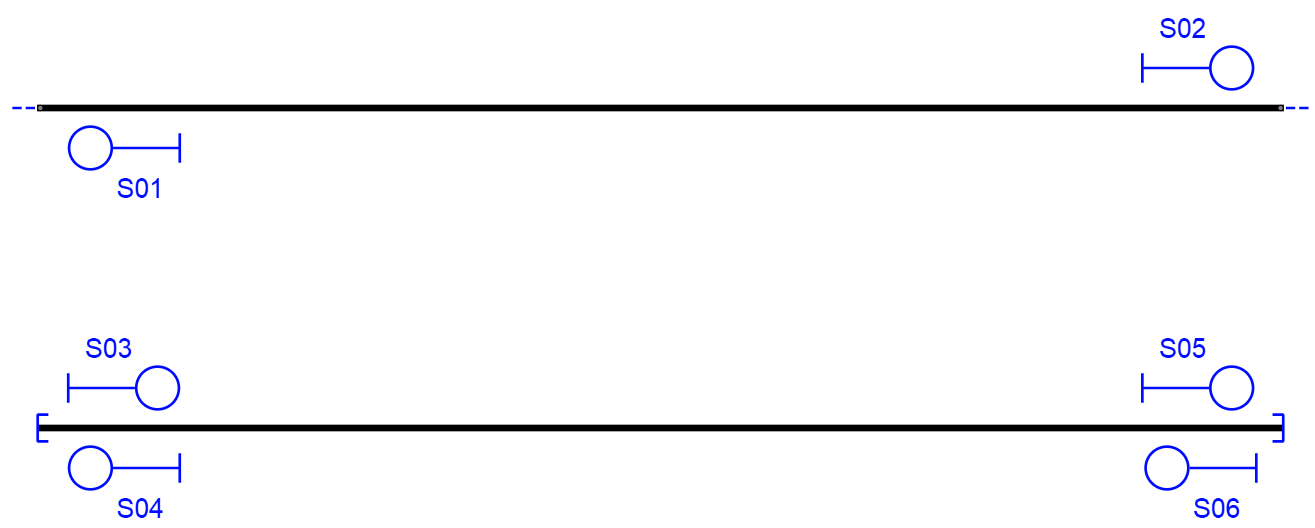
\includegraphics[width=1\textwidth]{Figuras/limites.PNG}
        \centering\caption{Señalamiento generado para finales de vía relativos y absolutos.}
        \label{fig:signal_border}
    \end{figure}
    
    El RNA detecta los \textit{line borders} en la vía superior y aplica el Algoritmo \ref{alg:lineBorder}, generando las señales de partida S01 para las formaciones que se mueven de derecha a izquierda y la señal de partida S02 para las formaciones que se mueven de izquierda a derecha, saliendo de la región mostrada en la Figura \ref{fig:signal_border}. Además, al detectar los \textit{buffer stops} en la vía inferior, el RNA aplica el Algoritmo \ref{alg:bufferStop}, generando cuatro nuevas señales. Las señales S04 y S05 son señales de parada para indicar a las formaciones que deben detenerse antes de colisionar con el final de la vía al transitar de derecha a izquierda o viceversa, respectivamente. Las señales S03 y S06 permiten a las formaciones reanudar su marcha en sentido contrario al que venían circulando, retomando su lugar en la red ferroviaria.
\subsection{Detectores}

\lipsum[1]

\begin{algorithm}[hbt!]
            \caption{Train detection elements algorithm}\label{alg:RJ}
            \DontPrintSemicolon
            %\SetAlgoLined
            \SetNoFillComment
            \LinesNotNumbered 
            \For { netElement WITH AxleCounters or RailJoints }
            {
                Track.Length = Length ( between RailJoints )\;
                \If { Track.Length $>$ FIXED\_LENGTH }
                {
                    [Signals] $\gets$ ADD circulation signal $>>>$\;
                    [Signals] $\gets$ ADD circulation signal $<<<$\;
                }
            }
            \KwResult{[Signals]} 
        \end{algorithm} 
\subsection{Plataformas ferroviarias}

    % Autoridad > derecho limitado a una porcion
    % Claridad > autoridad no ambigua
    % Anticipacion > avisar con antelacion
    % Granularidad > rutas cortas y funcionales
    % Terminalidad > avisar fin de via
    % Infraestructura > avisar de infraestructura
    % No bloqueo > circulacion fluida

    En la Sección \ref{sec:platform} definimos la clase platform que modela a las plataformas ferroviarias. Las plataformas ferroviarias son un punto del recorrido donde las formaciones pueden detenerse, algunas veces de forma opcional dependiendo el itinerario, para que los pasajeros desciendan y nuevos pasajeros puedan ascender. Claramente existe una limitación de autoridad, las formaciones necesitan un nuevo permiso para continuar circulando una vez alcanzada la plataforma. Permiso que será otorgado o negado según el estado del sistema a continuación del recorrido. Las plataformas ferroviarias suelen encontrarse en zonas pobladas, cerca de otras infraestructuras, zonas comerciales o residenciales, por lo que avisar con antelación al maquinista que debe disminuir la marcha y/o detenerse es esencial.

    Además, es posible que las formaciones convivan con otras formaciones que también hacen uso de la estación, por lo que las señales deben ser unívocas y claras. Algunas estaciones pueden contener fines de vías o ramificaciones hacia talleres u otros ramales, por lo que también se aplica el principio de terminalidad ($P_5$) y granuralidad ($P_4$). Finalmente, es importante el mantener una circulación fluida de las formaciones, de modo de no retrasar el itinerario de las formaciones que vienen detrás, por lo que se deberá aplicar el principio de no bloqueo ($P_7$).

    En el Algoritmo \ref{alg:PTF} definimos a la señal de partida como la única señal necesaria para operar una plataforma, asumiendo que la señal de ingreso de la misma será dada por otra instancia previa. De no existir otro elemento cercano por el cual se genere una señal, se puede asumir que la distancia a la plataforma es muy larga y, por lo tanto, se aplicaría el Algoritmo \ref{alg:RJ}, protegiendo a la plataforma. En el caso de que la vía sea bidireccional se añadiran señales de partida para ambos sentidos.

    \begin{algorithm}[hbt!]
        \caption{Algoritmo de generación de señalamiento para platforms.}\label{alg:PTF}
        \DontPrintSemicolon
        %\SetAlgoLined
        \SetNoFillComment
        \LinesNotNumbered 
        \For { netElement WITH Platform }
        {
            \tcc{Before leaving platform from left}
            [Signals] $\gets$ ADD departure signal $\gg\gg$\;
            \tcc{After leaving platform from right}
            [Signals] $\gets$ ADD departure signal $\ll\ll$\;
        }
        \KwResult{[Signals]} 
    \end{algorithm}

    Aplicando el Algoritmo \ref{alg:PTF} a un sistema de dos vías paralelas con plataformas pertenecientes a la misma estación obtenemos el resultado ilustrado en la Figura \ref{fig:signal_platform}.Se asumieron que ambas vías son bidireccionales, en caso contrario solo se generarían las señales S01 y S02.
    
    \begin{figure}[h!]
        \centering
        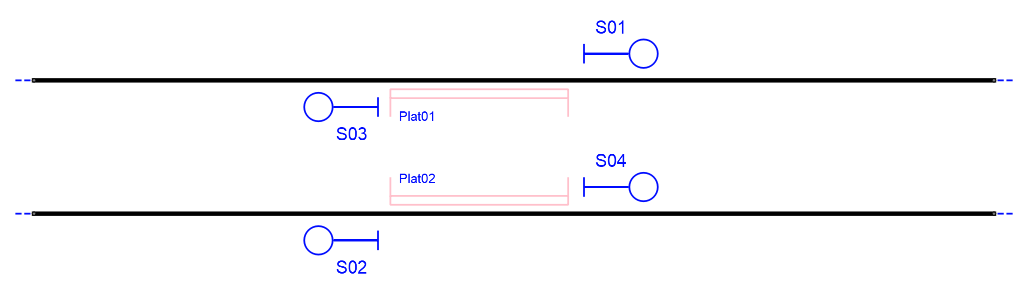
\includegraphics[width=1\textwidth]{Figuras/platforms.PNG}
        \centering\caption{Señalamiento generado para estaciones ferroviarias.}
        \label{fig:signal_platform}
    \end{figure}
    
    Una formación que circule de izquierda a derecha deberá detenerse antes de la señal S01, en caso de utilizar la vía superior, o antes de la señal S04, en caso de utilizar la vía inferior. Análogamente, las formaciones deberán detenerse antes de las señales S03 y S02 en el caso de transitar de derecha a izquierda por la vía superior o inferior respectivamente. Sólo cuando estas señales otorguen a la formación autoridad para circular podrán reanudar su marcha hasta la próxima señal disponible, fuera del alcance de lo ilustrado en la Figura \ref{fig:signal_platform}.
\subsection{Cruces de via}

\lipsum[1-2]

    \begin{algorithm}[hbt!]
        \caption{Level crossing algorithm}\label{alg:LC}
        \DontPrintSemicolon
        %\SetAlgoLined
        \SetNoFillComment
        \LinesNotNumbered 
        \For { netElement WITH LevelCrossing }
        {
            \tcc{Before reaching level crossing}
            [Signals] $\gets$ ADD circulation signal $>>>$\;
            \tcc{After leaving level crossing}
            [Signals] $\gets$ ADD circulation signal $<<<$\;
        }
        \KwResult{[Signals]} 
    \end{algorithm}

\lipsum[1]
\includegraphics{example-image}\\
\lipsum[1-2]
\subsection{Maquinas de cambios}
	\label{sec:signal_switches}
	
    % Autoridad > derecho limitado a una porcion
    % Claridad > autoridad no ambigua
    % Anticipacion > avisar con antelacion
    % Granularidad > rutas cortas y funcionales
    % Terminalidad > avisar fin de via
    % Infraestructura > avisar de infraestructura
    % No bloqueo > circulacion fluida
    
    En la Sección \ref{sec:switches} definimos la clase switches que modela a las máquinas de cambios. Las máquinas de cambios son de los elementos ferroviarios mas críticos de la red. Por lo tanto, se deberá aplicar al principio de infraestructura a cada una de sus entradas. Además, las máquinas de cambios actúan como una frontera entre las ramas principales de la red, donde se circula a mayor velocidad, y las ramas secundarias, donde se circula a una velocidad menor. Esto divide las rutas en dos o mas rutas, aplicando el principio de autoridad y granularidad. Finalmente, por el principio de no bloqueo, será necesario generar señales de diferente tipo para las ramas principales y las secundarias, priorizando las primeras. Esto puede cumplirse si otorgamos señales de circulación de tres o mas aspectos a la rama principal y señales de maniobra para utilizar una rama secundaria como salida o entrada de la red.
    
    En el Algoritmo \ref{alg:SW} definimos al punto de acceso de inicio como la vía desde la cual la trayectoria de la formación se bifurca, para lo cual se genera una señal de circulación para continuar por la rama principal y una señal de maniobra para acceder a la rama secundaria. Además, se añade una señal de circulación en la rama principal y una señal de maniobra en la rama secundaria, ambas en sentido contrario, para poder retornar al punto de inicio. 
    
    \begin{algorithm}[hbt!]
        \caption{Algoritmo de generación de señalamiento para Switches}\label{alg:SW}
        \DontPrintSemicolon
        %\SetAlgoLined
        \SetNoFillComment
        \LinesNotNumbered 
        \For { Switch in Switches }
        {
            \tcc{All signals must point to switch}
            \Switch{ Switch.Type }
            {
                \Case{Start}
                {
                    [Signals] $\gets$ ADD circulation signal\;
                    [Signals] $\gets$ ADD maneuver signal\;
                }
                \Case{Continue branch}
                {
                    [Signals] $\gets$ ADD circulation signal\;
                }
                \Case{Detour branch}
                {
                    [Signals] $\gets$ ADD maneuver signal\;
                }
            }   
        }
        \KwResult{[Signals]} 
    \end{algorithm}

    Aplicando el Algoritmo \ref{alg:SW} a un sistema de vías que se bifurcan obtenemos el resultado ilustrado en la Figura \ref{fig:signal_swithces}. Se asumieron que ambas vías son bidireccionales. En caso contrario, si el sentido de circulación es únicamente de bifurcación, las señales de retorno S02 y S03 no son necesarias. Si el sentido de circulación fuese de derecha a izquierda, las señales de inicio S01 no son necesarias.
    
    \begin{figure}[h!]
        \centering
        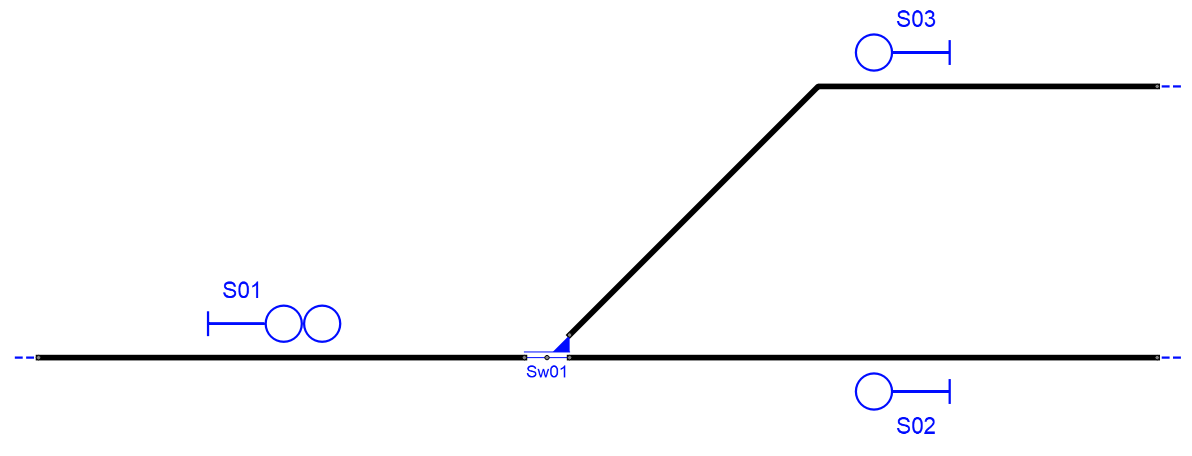
\includegraphics[width=1\textwidth]{Figuras/switches.PNG}
        \centering\caption{Señalamiento generado para cambios de vías.}
        \label{fig:signal_swithces}
    \end{figure}
    
    Una formación que circule de izquierda a derecha deberá detenerse antes de la señal S01. El aspecto mas cercano al poste de la señal S01 indicará si la formación puede circular por la vía principal, como se explicó en la Sección \ref{sec:signals}, previa confirmación por parte del sistema de enclavamiento de que el cambio Sw01 se encuentra en posición normal. De la misma forma, el sistema de enclavamiento confirmará que el cambio Sw01 se encuentra en posición reverso previo a habilitar la circulación por la vía secundaria mediante el aspecto mas alejado al poste de la señal S01.

    Una formación circulando de derecha a izquierda hará uso de las señales S02 y S03 si se encuentran en las vías principal o secundaria respectivamente. Las señales se habilitarán si el sistema de enclavamientos confirma que el cambio Sw01 se encuentra en la posición normal o reverso respectivamente y si no hay formaciones ocupando la vía de inicio donde se encuentra la señal S01, continuando su marcha hasta la próxima señal disponible, fuera del alcance de lo ilustrado en la Figura \ref{fig:signal_swithces}.    
    \section{Algoritmos de simplificación de señalamiento}
    \label{sec:simplificacion}

    % Autoridad > derecho limitado a una porcion
    % Claridad > autoridad no ambigua
    % Anticipacion > avisar con antelacion
    % Granularidad > rutas cortas y funcionales
    % Terminalidad > avisar fin de via
    % Infraestructura > avisar de infraestructura
    % No bloqueo > circulacion fluida
    
    Una vez finalizada la generación de señalamiento para cada elemento ferroviario, es necesario abordar el segundo miembro de la Fórmula \ref{frm:signal_1} explicada al comienzo de la Sección \ref{sec:generacion}. El señalamiento total para un sistema de N elementos ferroviarios será la suma de las señales necesarias para proteger a esos N elementos ferroviarios. Es inevitable que algunas señales se solapen con otras espacial o funcionalmente. Incluso algunas señales podrían contradecir a otras, oponiéndose al principio de claridad. La abundancia de señales puede hacer las rutas tan cortas que la autoridad estaría limitada a pequeñas porciones de la red, haciendo inviable una circulación fluida sobre la red.

    La simplificación del señalamiento se sustenta en dos algoritmos básicos: simplificación por herencia vertical y simplificación por herencia horizontal. Los dos algoritmos pueden aplicarse en cualquier orden, aunque los algoritmos de herencia vertical solamente se pueden aplicar en redes ramificadas que tengan máquinas de cambios. 

    El proceso de simplificación finaliza con el algoritmo de limpieza, que elimina todas las señales redundantes en base a un nivel de prioridades. Estas prioridades se relacionan directamente con qué elemento ferroviario el RNA intentaba proteger con esta señal, reteniendo la señal mas importante y eliminando el resto. También se combinan señales muy próximas en una vecindad y se borran señales contradictorias o redundantes, para obtener el señalamiento definitivo.    

 	\subsection{Algoritmo de simplificación por herencia vertical}
	\label{sec:vertical}
	% Autoridad > derecho limitado a una porcion
	% Claridad > autoridad no ambigua
	% Anticipacion > avisar con antelacion
	% Granularidad > rutas cortas y funcionales
	% Terminalidad > avisar fin de via
	% Infraestructura > avisar de infraestructura
	% No bloqueo > circulacion fluida
	
	Como se explicó en la Sección \ref{sec:switches}, una máquina de cambios bifurca la vía principal en dos: una vía que continúa la rama principal y otra vía que se convierte en una rama secundaria. Tanto la vía de continuación como la vía ramificada pueden tener otra máquina de cambios que, a su vez, vuelve a dividir el trazado ferroviario en dos. Esto incrementa más y más el nivel de complejidad de la red, añadiendo caminos divergentes al principal que luego, mas adelante, podrían, o no, volver a converger utilizando mas máquinas de cambios. Cada divergencia aporta un nivel de profundidad a la red, mientras que cada convergencia reduce en uno el nivel de profundidad.
	
	Una máquina de cambios que tiene en cualquiera de sus ramas divergentes el nodo de inicio de otra máquina de cambios a una distancia pequeña es un cambio compuesto. Los cambios compuestos requieren considerar a ambas máquinas de cambios como una sola, ya que es necesario posicionar ambos mecanismos para completar un movimiento. El ejemplo de La Figura \ref{fig:signal_vertical_1} ayudará a clarificar el concepto de cambios compuestos e introducir el Algoritmo de simplificación por herencia vertical.	

	\begin{figure}[H]
		\centering
		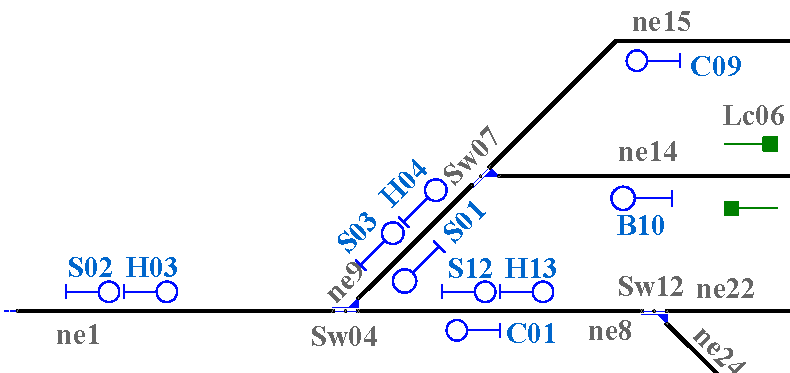
\includegraphics[width=1\textwidth]{Figuras/Figure8_Crop.pdf}
		\centering\caption{Señalamiento generado, simplificado por algoritmo de herencia vertical.}
		\label{fig:signal_vertical_1}
	\end{figure}
	
	En la Sección \ref{sec:signal_switches} se introdujo el Algoritmo \ref{alg:SW} que define la asignación de señalamiento para los cambios de vías: una señal de circulación (S) y de maniobra (H) para el nodo de inicio (S), una señal de circulación para el nodo de continuación (C) y una señal de maniobras para el nodo de desvío (B). El Algoritmo \ref{alg:SW} se aplicó de forma independiente a las máquinas de cambios Sw04, Sw07 y Sw12 y se obtuvo el señalamiento de la Figura \ref{fig:signal_vertical_1}. No obstante, el señalamiento generado no cumple con el principio de no bloqueo, al situar las señales S03, H04, B01, S12, H13 y C01 en las secciones correspondientes a los netElements ne9 y ne8. De esa manera, las formaciones podrían detenerse en esas secciones si las mencionadas señales presentasen un aspecto rojo.
	
	Una formación detenida en la sección correspondiente al \textit{netElement} ne9 no permitiría mover el cambio de vía Sw04, al tener parte de la formación aún en ne1. Tampoco permitiría accionar el cambio de vías Sw07 al no haber finalizado el movimiento. Análogamente, loa mismo ocurriría para una formación detenida en la sección correspondiente al \textit{netElement} ne8. Es necesario que el movimiento finalice, despejando las secciones y permitiendo que otras formaciones utilicen los cambios de vías Sw04 y Sw07, o cualquier combinación de mas de un cambio de vías.
	
	Para solucionar el problema expuesto, el RNA aplica el Algoritmo \ref{alg:vertical} de simplificación por herencia vertical para reposicionar las señales situadas en zonas conflictivas. A diferencia del señalamiento explicado en la Sección \ref{sec:generacion}, las señales que protegen a un cambio de vías B situado en una rama mas profunda de la red no se encuentran inmediatamente precediendo al cambio de vías B. Estas señales son movidas a ramas de menor profundidad con suficiente espacio físico para contenerlas, situándose precediendo a otro cambio de vías A que decimos que ha \emph{heredado} el señalamiento del cambio de vía B.
		
	\begin{algorithm}[H]
        \caption{Algoritmo de simplificación por herencia vertical}\label{alg:vertical}
        \DontPrintSemicolon
        %\SetAlgoLined
        \SetNoFillComment
        \LinesNotNumbered 
        \For{ each Signal protecting a Sw\_A }
        {
            \For{each Sw\_B != Sw\_A}
            {
                \tcc{Criteria \#0}
                \If{distance(Sw\_A,Sw\_B) $>$ MIN\_DISTANCE}
                {
                    Continue\;
                }
                \If{S in Sw\_A.Branch also in Sw\_B.Start} 
                {
                   \tcc{Criteria \#1}
                   \If{S points to Sw\_B.Start}
                   {
                        Move S to Sw\_A.Start\;
                   }
                   \tcc{Criteria \#2}
                   \If{S points to Sw\_A.Branch}
                   {
                        Move S to Sw\_B.Continue\;
                        Move S to Sw\_B.Branch\;
                   }
                }
                \If{S in Sw\_A.Continue also in Sw\_B.Start}
                {
                   \tcc{Criteria \#3}
                   \If{S points to Sw\_B.Start}
                   {
                        Move S to Sw\_A.Start\;
                   }
                   \tcc{Criteria \#4}
                   \If{S points to Sw\_A.Continue}
                   {
                        Move S to Sw\_B.Continue\;
                        Move S to Sw\_B.Branch\;
                   }
                }
            }
        
        }
        \KwResult{[Signals]} 
    \end{algorithm}

    Como puede apreciarse en el Algoritmo \ref{alg:vertical}, existen cinco criterios a considerar para aplicar la herencia vertical. El primer criterio es excluyente, si la distancia entre ambas máquinas de cambios supera un parámetro determinado entonces el algoritmo no se aplica, al existir suficiente distancia para situar el señalamiento sin generar obstrucciones debido a formaciones detenidas entre ambos. Cuando la distancia entre las máquinas de cambios es menor a lo esperado, se aplican los otros cuatro criterios, en función de que nodos conectan entre sí la vía que comparten.
    
    Definiendo al cambio de vías A como el cambio principal y el cambio de vías B como el cambio secundario situado en alguna de las ramificaciones del cambio de vías A, podemos diferenciar dos casos: que el señalamiento se encuentre en la rama de continuación del cambio de vías A o se encuentre en la rama de desvío. Además, este señalamiento puede estar apuntando al cambio de vías A o al cambio de vías B, protegiéndolo respectivamente. 
    
    El criterio para el desplazamiento del señalamiento busca cumplir el principio de Anticipación, el principio de Infraestructura y el principio de no bloqueo. Para eso, las señales son adelantadas, desplazándolas en sentido opuesto al que apuntan. Si el señalamiento se encuentra en la rama de desvío o continuación del cambio de vías A es indistinto, lo importante es a donde apuntan las señales. Si estas apuntan hacia el nodo de inicio del cambio de vías B, deben ser desplazadas, sin alterar su cantidad, hacia el nodo de inicio del cambio de vías A. 
    
    En el caso particular de que las señales en la zona conflictiva apunten hacia el cambio de vías A, tanto a su nodo de desvío como al nodo de continuidad, las mismas deberían moverse en sentido contrario al que apuntan. Sin embargo, en esa dirección la red se ramifica en dos debido al cambio de vías B. En este caso, las señales mueven duplicadas, a la rama de continuación y a la rama de desvío del cambio de vías B, en su totalidad.
    
    Aplicando el Algoritmo \ref{alg:vertical} de herencia vertical al ejemplo de la Figura \ref{fig:signal_vertical_1} obtenemos el señalamiento de la Figura \ref{fig:signal_vertical_2}. Las señales S03, H04, B01, S12, S13 y C01 serán adelantadas para despejar las secciones correspondientes a los netElements ne9 y ne8. Debido a esto, los tres cambios de vías se usarán de forma complementaria, creando los siguientes cambios compuestos: $Sw_{04}^R+Sw_{07}^N$, $Sw_{04}^R+Sw_{07}^R$, $Sw_{04}^N+Sw_{12}^N$ y $Sw_{04}^N+Sw_{12}^R$. Los cuales se leen, considerando el ejemplo del cambio compuesto $Sw_{04}^R+Sw_{07}^N$, de la siguiente manera: el cambio de vías Sw04 en posición normal y el cambio de vías Sw07 en posición reversa.
    
    \begin{figure}[H]
    	\centering
    	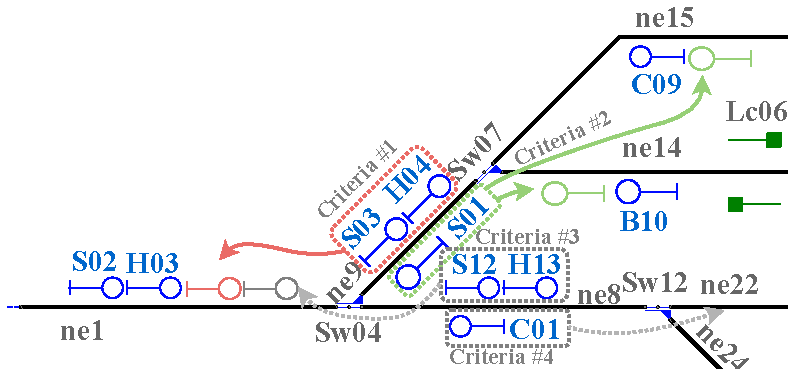
\includegraphics[width=1\textwidth]{Figuras/Figure9_Crop.pdf}
    	\centering\caption{Señalamiento generado, simplificado por algoritmo de herencia vertical.}
    	\label{fig:signal_vertical_2}
    \end{figure}
    
    En el caso de las señales S03 y H04 que apuntan al nodo de inicio del cambio de vías Sw07, son desplazadas en sentido contrario al que apuntan, aplicando el criterio \#1. Estas señales son movidas hasta el nodo de continuación del cambio de vías Sw04, correspondiente al netElement ne1, protegiendo el inicio del cambio compuesto $Sw_{04}^R+Sw_{07}^N$ y $Sw_{04}^R+Sw_{07}^R$ . A estas señales se le suman las señales S12 y H13 situadas en la sección correspondiente al netElement ne8 que, aplicando el criterio \#3, son desplazadas al nodo de inicio del cambio de vías Sw04, protegiendo el inicio del cambio compuesto $Sw_{04}^N+Sw_{12}^N$ y $Sw_{04}^N+Sw_{12}^R$.
    
    La señal B01 apunta al nodo de desvío del cambio de vías Sw04 y, por el criterio \#2, debe ser duplicada y movida. Una señal se posiciona en la sección correspondiente al netElement ne15 y la otra a la sección asociada al netElement ne14. De esta manera, la señal S01a y S01b seguirán protegiendo el nodo de desvío del cambio de vías Sw04, pero previamente tendrán que hacer uso del cambio de vías Sw07 en cualquiera de sus dos posiciones, protegiendo los nodos de cambio y continuación del cambio compuesto $Sw_{04}^R+Sw_{07}^N$ y $Sw_{04}^R+Sw_{07}^R$. De igual manera, la señal C01 es movida y duplicada a las secciones correspondientes a los netElements ne22 y ne24, debido al criterio \#4. Estas nuevas señales C01a y C01b continúan protegiendo el nodo de continuación del cambio de vías Sw04, pero ahora deberán, adicionalmente, hacer uso del cambio de vías Sw12, protegiendo los nodos de continuación y desvío del cambio compuesto $Sw_{04}^N+Sw_{12}^N$ y $Sw_{04}^N+Sw_{12}^R$.
    
    El Algoritmo \ref{alg:vertical} de herencia vertical es exitoso a la hora de despejar las zonas críticas entre cambios de vías muy cercanos. No obstante, también incrementa la cantidad de señales, como en el caso de las señales S01 y C01 al ser desplazadas en sentido divergente por los cambios de vías Sw07 y Sw12. Además, el Algoritmo \ref{alg:vertical} de herencia vertical no es aplicable solo a una dupla de cambios de vías, sino que puede ser aplicado para cualquier conjunto de cambios de vías. Esto provoca que las señales se hereden de forma iterativa hasta encontrar un cambio de vías con suficiente espacio para albergar las señales. Debido a esto, la cantidad de señales al comienzo de un cambio de vías previo a una ramificación profunda de la red tendrá una gran cantidad de señales.
    
    En el caso del ejemplo de las Figuras \ref{fig:signal_vertical_1} y \ref{fig:signal_vertical_2}, el algoritmo concluye con seis señales en el nodo de inicio de los cuatro cambios compuestos. Estas seis señales deberán habilitar cuatro caminos a transitar desde ne1: hacia ne15, hacia ne14, hacia ne22 y hacia ne24. Es claro que, teniendo mas señales que caminos a habilitar, será necesario un algoritmo de limpieza de señales duplicadas y/o que ya no tengan una utilidad en el señalamiento. El proceso de simplificación es explicado en profundidad en la Sección \ref{sec:limpieza}.
    \subsection{Algoritmo de herencia horizontal}

\lipsum[1]

\begin{algorithm}[hbt!]
        \caption{Horizontal inheritance algorithm}\label{alg:horizontal}
        \DontPrintSemicolon
        %\SetAlgoLined
        \SetNoFillComment
        \LinesNotNumbered 
        \For{ each netElement }
        {
            \For{ each object in netElement }
            {
                \If{dist(Obj\_A,Obj\_B) $<$ MIN\_DISTANCE }
                {
                    move\_signals\_between(Obj\_A,Obj\_B)
                }
            }
        }
        \KwResult{[Signals]} 
    \end{algorithm}

    \lipsum[1-3]
    \subsection{Limpieza de señales}
	\label{sec:limpieza}

	% Autoridad > derecho limitado a una porcion
	% Claridad > autoridad no ambigua
	% Anticipacion > avisar con antelacion
	% Granularidad > rutas cortas y funcionales
	% Terminalidad > avisar fin de via
	% Infraestructura > avisar de infraestructura
	% No bloqueo > circulacion fluida
	
	El Algoritmo \ref{alg:vertical} de simplificación por herencia vertical y el Algoritmo \ref{alg:horizontal} de simplificación por herencia horizontal tienen diferentes efectos en la cantidad de señales totales. El Algoritmo de herencia horizontal mueve las señales entre elementos cuando no existe suficiente espacio entre ellos. Sin embargo, el Algoritmo de herencia vertical duplica la cantidad de señales si se aplica el criterio \#2 o el \#4. Todos los algoritmos que utiliza el RNA pueden aplicarse de forma iterativa si las condiciones lo permiten, pero particularmente el Algoritmo \ref{alg:vertical} duplicará las señales por cada nivel de profundidad de la red ferroviaria. Esto llevará a tener mas señales que las necesarias en algunos netElements. Este exceso de señales deben eliminarse para mantener una proporción uno a uno entre una señal y una funcionalidad específica. El Algoritmo \ref{alg:reduction} se ocupa de la limpieza de las señales que se encuentran muy próximas entre si, eliminando siempre las que tengan menor prioridad. 

	\begin{algorithm}[H]
        \caption{Signal reduction algorithm}\label{alg:reduction}
        \DontPrintSemicolon
        %\SetAlgoLined
        \SetNoFillComment
        \LinesNotNumbered 
        Sources = $\{$ T,L,S,B,P,C,J,X $\}$\;
        \For{ Sig\_A \& Sig\_B in [Signals]}
        {
            \If{ A != B  \& Sig\_A.From == Sig\_B.From }
            {
             Signalling\_zones.Pos = detect\_next\_dangers ( Sig\_A )\;
             A.Pos,B.Pos = Sig\_A.Pos,Sig\_B\;
             Safe = zone\_between(Signalling\_zones.Pos,A.Pos,B.Pos)\;
                 \If{ NOT safe }
                 {
                    \If{ $|A.Pos,B.Pos|$ $<$ MIN\_DISTANCE }
                    {
                        \If{ Sig\_A \& Sig\_B same orientation }
                        {
                            \If{ Sig\_A \& Sig\_B same direction }
                            {
                                \If { Sig\_A \& Sig\_B type "Circ" }
                                {
                                    \If{ Sig\_A.Idx $<$ Sig\_B.Idx }
                                    {
                                        delete Sig\_B  else Sig\_A
                                    }
                                    %{
                                    %    delete( Sig\_A )
                                    %}
                                }
                            }
                        }
                        \If{ Sig\_A \& Sig\_B different source}
                        {
                            delete\_lowest\_priority( Sig\_A,Sig\_B )\;
                        }
                    }
                }
            }
        }
        \KwResult{[Signals]} 
    \end{algorithm}

	La prioridad es definida según el origen de cada señal. Como se explicó en la Sección \ref{sec:generacion}, las señales pueden tener diferentes etiquetas en función de que elemento ferroviario están protegiendo. Las señales S C B y H protegen los cambios de vías, las señales P a las plataformas, las señales J a las junturas, las señales X a los cruces de vías. Todas ellas son señales de circulación, salvo las señales B y H que son de maniobras. La prioridad mas alta fue asignada a las señales que protegen los finales de vía absolutos (T) y relativos (L) porque son las únicas señales de parada que no pueden ser reemplazadas por señales menos restrictivas. 
	
	Esto no significa que todas las señales que protegen los finales de vía (T) eliminarán todas las señales de los pasos a nivel (X), sino que de tener otra señal cercana del mismo tipo que apunte en la misma dirección y sentido, pero de mayor prioridad, será ésta quien cumpla la función de proteger al paso a nivel. Las señales pueden tener diferentes roles, como ser señales de parada, de circulación, de partida o maniobra. Las señales de parada son absolutas y se utilizan en finales de vía, mientras que las señales de partida se utilizan para reiniciar la marcha de la formación. Las primeras poseen un aspecto rojo, mientras que las segundas pueden tener hasta tres aspectos. Las señales de circulación poseen tres aspectos y permiten velocidades mas altas en las ramas principales de la red. Las señales de maniobra poseen solamente dos aspectos y son utilizadas en los desvíos, tanto en ramas divergentes como en convergentes.
	
	En el caso de que dos señales que tengan igual dirección, sentido y origen, pero no tengan una región de señalamiento entre ellas, deban ser simplificadas. En este caso, se decidió eliminar la señal con índice mas alto. Esto se debe a que, una vez generado el señalamiento para cada elemento, las señales de mayor índice serán las producidas por los Algoritmos de herencia horizontal y vertical, que tiendan a añadir señales que con mucha probabilidad deben ser eliminadas a posteriori.
	
    Es importante resaltar que la asignación de prioridades es de vital importancia para la seguridad. Por ejemplo, que las señales B tengan mayor prioridad que las señales P. Si la plataforma se encuentra lo suficientemente alejada de un cambio de vías, una señal de maniobra que protege el cambio de vías no puede reemplazar una señal de circulación que protege a una plataforma porque siempre habrá una plataforma entre ambos y, por lo tanto, una región de señalamiento. Sin embargo, si la plataforma se encuentra lo suficientemente cerca del cambio de vías, la señal de maniobras B se movería hacia la región de señalamiento donde se encuentra la señal de circulación P, debido al Algoritmo \ref{alg:horizontal} de herencia horizontal por el cual dos elementos ferroviarios muy próximos combinan sus regiones de señalamiento. Por lo tanto, la señal B de dos aspectos reemplazara a la señal P de tres aspectos, reduciendo la velocidad máxima permitida en esa zona de la red ferroviaria, incrementando la seguridad de la red.	
    \section{Generacion de tablas de enclavamiento}

\lipsum[1]

\begin{algorithm}[hbt!]
        \caption{Route detection algorithm}\label{alg:routes}
        \DontPrintSemicolon
        %\SetAlgoLined
        \SetNoFillComment
        \LinesNotNumbered 
        Routes = [], route = 0\;
        \For{ start in [Signals] }
        {
            \tcc{Find manoeuvre and circulation signals}
            \If{ start != "Stop" }
            {
                dir = start\_sig.Direction\;
                \tcc{Find next signal w/ same direction}
                
                end = find\_next\_signal(start,[Signals])\;

                [paths] = find(start.node,end.node,graph)\;
                
                \For{ node in [paths] }
                {
                    \tcc{Find rail objects within path}
                    sws = find(graph[node],switches)\;
                    lc = find(graph[node],levelCrossings)\;
                    ptf = find(graph[node],platforms)\;
                    %route ++\;
                    Routes[route++] = $\{$start,end,dir,node,sws,lc,ptf$\}$\;
                }
            }
        }
        \KwResult{[Routes]} 
    \end{algorithm}
    \section{Validacion de tablas de enclavamiento}

\lipsum[1]
    \section{Validación de principios de señalamiento ferroviario}
	\label{sec:validar_principios}
	
	% Autoridad > todas las rutas combinadas cubren toda la traza ferroviaria.
	% Claridad > autoridad no ambigua.
	% Anticipacion > avisar con antelacion.
	% Granularidad > rutas cortas y funcionales.
	% Terminalidad > avisar fin de via.
	% Infraestructura > avisar de infraestructura.
	% No bloqueo > circulacion fluida.
				
	En esta sección se abordará el proceso de validación de cada uno de los principios ferroviarios establecidos en la Sección \ref{sec:principios}, como parte del proceso expuesto en la Sección \ref{sec:validacion}. Para ello, serán abordados de manera genérica cada uno de los principios de señalamiento junto con el algoritmo que el RNA utiliza para validarlo, previo a exportar el señalamiento generado.
	
	\subsection{Validación del principio de autoridad}
		% Autoridad > todas las rutas combinadas cubren toda la traza ferroviaria.
		
		El principio de autoridad radica en que las rutas otorgan a las formaciones un permiso de uso limitado para circular por las vías. No obstante, la combinación de todas las autoridades disponibles de ser otorgadas deben cubrir la totalidad de la traza ferroviaria. Es decir, no debe existir ninguna sección de vía que se encuentre fuera del alcance de las rutas y, por lo tanto, aislada de la red. Puede darse el caso de que una sección de vía tenga una ruta de entrada o de salida, pero no ambas. También puede darse el caso de que la sección de vía sea transitada, pero no sea ni inicio ni final de ninguna ruta.
		
		El RNA utiliza el Algoritmo \ref{alg:ppio_autoridad} para validar el principio de autoridad comparando los netElements alcanzados por las rutas disponibles, con la lista de netElements potenciales de ser alcanzados. Esta última salvedad deja fuera las secciones de vías que preceden a una señal de circulación posterior a un final de vía relativo (lineBuffer). Esto se realiza ya que estas secciones de vía son transitadas por rutas fuera de la locación bajo análisis, rutas que terminan en la señal de circulación mencionada.

		\begin{algorithm}[hbt!]
			\caption{Algoritmo de validación del principio de autoridad.}\label{alg:ppio_autoridad}
			\DontPrintSemicolon
			%\SetAlgoLined
			\SetNoFillComment
			\LinesNotNumbered 
			Validated = False\;
			$\{$Routes$\}$, $\{$netElements$\}$ without netElements with lineBuffer\; 
			\tcc{Validate that every route covers all the railway tracks.}
			\For{route in $\{$Routes$\}$}
			{
				\If{route[begin] in $\{$netElements$\}$}
				{
					Remove route[begin] from $\{$netElements$\}$\; 
				}
				\If{route[end] in $\{$netElements$\}$}
				{
					Remove route[end] from $\{$netElements$\}$\; 
				}
				\For{track in route[paths]}
				{
					\If{track in $\{$netElements$\}$}
					{
						Remove track from $\{$netElements$\}$\; 
					} 
				}
			}
			\If{$\{$netElements$\}$ is Empty}
			{
				Validated = True\; 
			} 
			\KwResult{Validated} 
		\end{algorithm}
		
		Se asume inicialmente que la validación es fallida por defecto. Si al finalizar el Algoritmo \ref{alg:ppio_autoridad} no existe ningún netElement remanente en la lista, se considera que la validación es exitosa.	
			
	\subsection{Validación del principio de claridad}
		% Claridad > autoridad no ambigua
		
		El principio de claridad radica en que el señalamiento no posee señales ambiguas. Es decir, no existen dos rutas distintas que otorguen autoridad sobre las mismas secciones de vía, en el mismo sentido, utilizando la misma infraestructura. En otras palabras, las rutas en una misma dirección y sentido no se solapan, cada una comienza donde otra ha terminado.
		
		El RNA utiliza el Algoritmo \ref{alg:ppio_claridad} para validar el principio de claridad, generando una red de grafos dirigidos. La misma se constituye utilizando todas las rutas definidas por el RNA como aristas, y a los netElements que conectan como nodos de la red. Si se detecta que existen dos rutas R$^{\prime}$ y R$^{\prime\prime}$ que conectan dos nodos A y B en el mismo sentido, utilizando la misma infraestructura, entonces se dice que las rutas son ambiguas y el principio de claridad no se cumple.
		
		\begin{algorithm}[hbt!]
			\caption{Algoritmo de validación del principio de claridad.}\label{alg:ppio_claridad}
			\DontPrintSemicolon
			%\SetAlgoLined
			\SetNoFillComment
			\LinesNotNumbered 
			Validated = False\;
			$\{$Routes$\}$\; 
			\tcc{Validate that every netElement is reached by one route only.}
			\For{route in $\{$Routes$\}$}
			{
				begin = route[begin]\;
				end = route[end]\;
				index = route[index] \;
				direction = route[direction]\;
				digraph = create\_digraph(begin,end,index,direction)\;	
			}
			\If{digraph has no redundant routes}
			{
				Validated = True\;
			}
			\KwResult{Validated} 
		\end{algorithm}
		
		Aunque el orden de validación de los principios de señalamiento es indistinto, la confirmación de que las señales son suficientes para alcanzar toda la red (Principio de autoridad) y de que no existen señales ambiguas (Principio de claridad) facilita las siguientes validaciones. Esto se debe a que, con estas dos comprobaciones, ya sabemos que contamos con la mínima cantidad de señales para recorrer la red de forma unívoca, garantizando la correcta logística de la red. Los siguientes principios son necesarios para validar la seguridad del señalamiento generado por el RNA.
		
	\subsection{Validación del principio de anticipación}
		% Anticipacion > avisar con antelacion
		
		El principio de anticipación radica en que existe una señal previo a cada peligro, situada en la zona de señalamiento. Una zona señalamiento puede estar próxima a una curva, al final de la traza ferroviaria o en las inmediaciones de un paso a nivel, una estación, un cambio de vías o cualquier infraestructura ferroviaria a ser protegida. En otras palabras, el señalamiento debe estar distribuido de tal manera que entre dos señales que constituyen una ruta exista un único peligro o situación que quiera la atención del conductor.
		
		El RNA utiliza el Algoritmo \ref{alg:ppio_anticipacion} para validar el principio de anticipación, detectando las regiones de señalamiento como zonas peligro peligrosas, producto del trazado ferroviario (curvas, finales de vía) o de la infraestructura ferroviaria (plataformas, pasos a nivel, etc.). 
		
		\begin{algorithm}[hbt!]
			\caption{Algoritmo de validación del principio de anticipación.}\label{alg:ppio_anticipacion}
			\DontPrintSemicolon
			%\SetAlgoLined
			\SetNoFillComment
			\LinesNotNumbered 
			Validated = True, $\{$Dangers$\}$ = None\;
			$\{$Routes$\}$, $\{$Track$\}$\; 
		
			\tcc{Validate that each danger is protected by the signalling.}
			
			\For{curve in $\{$Tracks$\}$}
			{
				$\{$Dangers$\}$ $\Leftarrow$ ADD curve
			}
			
			\For{element in $\{$Infraestructure$\}$}
			{
				$\{$Dangers$\}$ $\Leftarrow$ ADD element
			}
			
			\For{danger in $\{$Dangers$\}$}
			{
				
				\For{track going into danger}
				{
					\If{track has signal AND signal points to danger}
					{
						Continue\;
					}
					\Else
					{
						Validated = False\; 
						Stop iterations\;
					}
				}	
			}
			
			\KwResult{Validated} 
		\end{algorithm}
		
		A continuación, el Algoritmo \ref{alg:ppio_anticipacion} comprueba que existe una señal para cada dirección del peligro, apuntando en el sentido del mismo. Garantizando de esta forma, que previo a cada peligro inicie o finalice una ruta, en caso de que la ruta sea segura de ser transitada o no, respectivamente.
		
		Una sola región de señalamiento que tenga una de sus entradas sin proteger por una señal es suficiente para que el Algoritmo \ref{alg:ppio_anticipacion} devuelva un resultado negativo. Si todas las entradas de cada región de señalamiento están protegidas por una señal, entonces el principio de anticipación se encuentra cumplido. En el caso de que los elementos ferroviarios se encuentren muy próximos, por herencia horizontal, se consideran un único elemento y sus regiones de señalamiento se simplifican como se explicó en la Sección \ref{sec:horizontal}.
		
	\subsection{Validación del principio de granularidad}
		% Granularidad > rutas cortas y funcionales
		
		El principio de granularidad radica en que las rutas deben ser lo suficientemente cortas como para permitir una logística flexible, pero no tan cortas como para no tener ninguna funcionalidad real. Consideramos, por lo tanto, que el señalamiento debe estar distribuido de tal forma que las rutas tengan una funcionalidad básica. Entre éstas funciones tenemos el uso de un elemento ferroviario específico (o conjunto de elementos ferroviarios, si están muy próximos) o la subdivisión de rutas cuyos tramos originales eran demasiado extensos.
		
		El RNA utiliza el Algoritmo \ref{alg:ppio_granularidad} para validar el principio de granularidad, analizando que elementos ferroviarios se encuentran contenidos en cada ruta y la distancia entre las señales que conforman la misma. Se recorre el listado de rutas generadas por el RNA, que ya establece los elementos contenidos en las rutas, las señales que las definen y la posición de las mismas. En cada ruta se analiza si existen elementos ferroviarios que justifiquen la existencia de la ruta y si el largo de la misma se encuentra entre un rango mínimo y máximo estipulado. Si alguna de estas condiciones se cumple, entonces se procede a analizar la siguiente ruta. En caso contrario, el Algoritmo \ref{alg:ppio_granularidad} finaliza de forma negativa. Si todas las rutas analizadas superan el proceso, entonces el principio de granularidad ha sido validado exitosamente.
		
		\begin{algorithm}[hbt!]
			\caption{Algoritmo de validación del principio de granularidad.}\label{alg:ppio_granularidad}
			\DontPrintSemicolon
			%\SetAlgoLined
			\SetNoFillComment
			\LinesNotNumbered 
			Validated = True\;
			$\{$Routes$\}$\; 
			\tcc{Validate that each route has a purpose and a min/max length.}
			\For{route in $\{$Routes$\}$}
			{
				\If{MIN > route[length] > MAX OR route[elements] == None}
				{
					Validated = False\; 
					Stop iterations\;
				}				
			}
			\KwResult{Validated} 
		\end{algorithm}
		
		Si la ruta es demasiado pequeña o demasiado larga, la validación finaliza de forma negativa. Si la ruta tiene un tamaño adecuado pero no contiene ningún elemento relevante de ser protegido, también se rechaza la validación. En caso contrario, si todas las rutas cumplen el criterio entonces se da por validado el principio de granularidad.
		
	\subsection{Validación del principio de terminalidad}
		% Terminalidad > avisar fin de via
		
		El principio de terminalidad radica en que el señalamiento debe indicar, sin excepciones, el final de cada rama del trazado ferroviario, sin importar si es un final relativo u absoluto. Como se explicó en la Sección \ref{sec:bufferstop}, tanto los finales de vía relativos como los absolutos necesitan una señal de parada que permita habilitar la salida de la formación de la locación bajo estudio. Además, los finales de vía absolutos requieren de una señal de partida para reiniciar la marcha de la formación en la dirección contraria, retomando el recorrido dentro de la traza ferroviaria.	
		
		El RNA utiliza el Algoritmo \ref{alg:ppio_terminalidad} para validar el principio de terminalidad, recorriendo cada una de las rutas generadas y analizando aquellas que culminan o empiezan en un final de vía. Una vez detectadas las rutas que posean lineBorders o bufferStops, se procede a analizar que clase de señales poseen. Si son compatibles con las condiciones indicadas en la Sección \ref{sec:bufferstop}, entonces se continúa analizando con la siguiente ruta. Caso contrario, la validación termina de forma negativa. Si todas las rutas analizadas superan el proceso, entonces el principio de terminalidad ha sido validado exitosamente.
		
		\begin{algorithm}[hbt!]
			\caption{Algoritmo de validación del principio de terminalidad.}\label{alg:ppio_terminalidad}
			\DontPrintSemicolon
			%\SetAlgoLined
			\SetNoFillComment
			\LinesNotNumbered 
			Validated = True\;
			$\{$Routes$\}$\; 
			\tcc{Validate that each lineBorder and BufferStop have protective signals}
			\For{route in $\{$Routes$\}$}
			{
				\If{lineBorder in route[element] and route goes to lineBorder}
				{
					\If{signal is not route[end]}
					{
						Validated = False\;
					}
				}
				
				\If{bufferStop in route[element]}
				{
					\If{route goes to bufferStop and signal is not route[end]}
					{
						Validated = False\;
					}
					\If{route start from bufferStop and signal is not route[begin]}
					{
						Validated = False\;
					}
				}
			}
			
			\KwResult{Validated} 
		\end{algorithm}
		
		Este principio es el más sencillo de validar positivamente ya que, por como fue diseñado el RNA, tanto los lineBorder y los bufferStop siempre tendrán señalamiento y dichas señales tienen la máxima prioridad, por lo que no pueden simplificarse con otras señales. No obstante, si el usuario eligiendo de forma explícita no generar señales para estos elementos ferroviarios entonces este principio de señalamiento podría no cumplirse.		
				
	\subsection{Validación del principio de infraestructura}
		% Infraestructura > avisar de infraestructura
		
		El principio de infraestructura radica en que el señalamiento debe proteger, sin excepciones, toda infraestructura ferroviaria crítica, tales como las plataformas y los pasos a nivel. Con excepción de los cambios de vías, que son cubiertos por el principio de no bloqueo. La infraestructura deberá estar protegida por el señalamiento tal como se explicó en la Sección \ref{sec:platform} y la Sección \ref{sec:crossing}, permitiendo a las formaciones detenerse en las plataformas y antes de los pasos a nivel, respectivamente.

		El RNA utiliza el Algoritmo \ref{alg:ppio_infraestructura} para validar el principio de infraestructura, recorriendo cada una de las rutas generadas y analizando aquellas que atraviesan paso a nivel o que inician o finalizan en una plataforma. 
		
		\begin{algorithm}[hbt!]
			\caption{Algoritmo de validación del principio de infraestructura.}\label{alg:ppio_infraestructura}
			\DontPrintSemicolon
			%\SetAlgoLined
			\SetNoFillComment
			\LinesNotNumbered 
			Validated = True\;
			$\{$Routes$\}$\; 
			\tcc{Validate that each platform and crossing have protective signals}
			\For{route in $\{$Routes$\}$}
			{
				\If{platform in route[element]}
				{
					\If{route goes across platform and signal is not route[end]}
					{
						Validated = False\;
					}
					\If{route start from platform and signal is not route[begin]}
					{
						Validated = False\;
					}
				}
				
				\If{levelCrossing in route[element]}
				{
					\If{route goes to levelCrossing and signal is not route[end]}
					{
						Validated = False\;
					}
					\If{route start before levelCrossing and signal is not route[begin]}
					{
						Validated = False\;
					}
				}
			}
			
			\KwResult{Validated} 
		\end{algorithm}
		
		Una vez detectadas las rutas, se procede a analizar que clase de señales poseen.  Si son compatibles con las condiciones indicadas en la Sección \ref{sec:platform} y la Sección \ref{sec:crossing}, entonces se continúa analizando con la siguiente ruta. Caso contrario, la validación termina de forma negativa. Si todas las rutas analizadas superan el proceso, entonces el principio de infraestructura ha sido validado exitosamente.
		
		En el caso de que las plataformas y los pasos a nivel se encuentren muy próximos, por la simplificación de señalamiento por herencia horizontal explicada en la Sección \ref{sec:horizontal}, igualmente el Algoritmo \ref{alg:ppio_infraestructura} buscará las señales mas próximas al nuevo elemento ferroviario compuesto. De esta manera, al analizar todas las rutas exitosamente, es posible validar el señalamiento que protege a los elementos ferroviarios críticos, cumpliendo el principio de infraestructura.
		
	\subsection{Validación del principio de no bloqueo}
		% No bloqueo > circulacion fluida
		
		El principio de no bloqueo radica en que el señalamiento debe proteger los cambios de vías en sus tres direcciones: inicio,normal y desvío, como se explica en la Sección \ref{sec:switches}. A su vez, debe garantizarse que los cambios compuestos no tengan señales intermedias, para evitar que las formaciones se detengan en zonas críticas, bloqueando los cambios de vías para otras formaciones que las requieran, como se explica en la Sección \ref{sec:vertical}.
		
		El RNA utiliza el Algoritmo \ref{alg:ppio_nobloqueo} para validar el principio de no bloqueo, recorriendo la lista de máquinas de cambios. El primer paso es agrupar en tres listas distintas todos los netElements de cada cambio de vía según su dirección: inicio, normal y desvío. Luego, son removidas de las listas de inicio y normal todos los netElements que también pertenezcan a la lista de desvío. De esta manera, el algoritmo contempla a los cambios compuestos productos de la simplificación por herencia vertical (ver Sección \ref{sec:vertical}). 
		
	
		
		\begin{algorithm}[hbt!]
			\caption{Algoritmo de validación del principio de no bloqueo.}\label{alg:ppio_nobloqueo}
			\DontPrintSemicolon
			%\SetAlgoLined
			\SetNoFillComment
			\LinesNotNumbered 
			Validated = False\;
			$\{$Switches$\}$\;
			switch\_start = [], switch\_normal = [], switch\_branch = [], critical = []\;
			\tcc{Validate that each switch have protective signals}
			
			\tcc{List netElements for each side of each switch}
			
			\For{sw in $\{$Switches$\}$}
			{
				switch\_start $\leftarrow$ ADD sw[netElement] for 'Start'\;
				switch\_normal $\leftarrow$ ADD sw[netElement] for 'Normal'\;
				switch\_branch $\leftarrow$ ADD sw[netElement] for 'Branch'\;
			}	
			
			\tcc{Remove netElements that also belongs to a branch}
			\For{sw in $\{$Switches$\}$}
			{
				switch\_start $\leftarrow$ REMOVE netElement if in switch\_branch\;
				switch\_normal $\leftarrow$ REMOVE netElement if in switch\_branch\;
				critical $\leftarrow$ ADD netElement in switch\_branch AND (switch\_start OR switch\_normal)\;
			}	
			
			\tcc{Remove the netElements that have signals}
			\For{netElement that has a signal}
			{
				\If{netElement in unprotected\_switch\_start}
				{
					switch\_start $\leftarrow$ REMOVE netElement\;
				}
				
				\If{netElement in unprotected\_switch\_normal}
				{
					switch\_normal $\leftarrow$ REMOVE netElement\;
				}
			}
			
			\tcc{Final condition}
			\If{switch\_start == [ ] AND switch\_normal == [ ] AND critical has no signals}
			{
				Validated = True\;
			}
			
			\KwResult{Validated} 
		\end{algorithm}
		
		A continuación, se remueven de las listas de inicio y normal todos los netElements que tienen una señal apuntando hacia el cambio de vías. Finalmente, si ambas listas se encuentran vacías y los netElements de la lista de cambios que también perteneciesen a las listas de inicio y normal originales no tienen señales, entonces el principio de no bloqueo ha sido validado exitosamente.
		
	Una vez que todos los principios de señalamiento ferroviario han sido validados podemos afirmar que el señalamiento generado por el RNA es seguro y cumple con todos los requisitos planteados en la Sección \ref{sec:principios}. Dicho señalamiento deberá ser implementado por el Generador Automático de Códigos en VHDL (ACG), explicado en profundidad en la Sección \ref{sec:ACG}.
